% !TeX root = Probability-Theory.tex
\documentclass{report}
%%%%%%%%%%%%%%%%%%%%%%%%%%%%%%%%%
% PACKAGE IMPORTS
%%%%%%%%%%%%%%%%%%%%%%%%%%%%%%%%%
\usepackage{svg}
\usepackage{datetime2}
\usepackage{fontspec-xetex}
\usepackage{xeCJK}
\usepackage{fancyhdr}
\usepackage{twemojis}
\usepackage{metalogo}
\usepackage{marginnote}
\usepackage{wrapfig}
\setCJKmainfont[ItalicFont=LXGW WenKai Mono GB, BoldFont=Hiragino Sans GB W6]{BabelStone Han}
\setCJKmonofont{Sarasa Fixed Slab SC}
\setCJKsansfont{Sarasa Gothic SC}
\setCJKmathfont{BabelStone Han}
\setCJKfamilyfont{jarm}{IPAmjMincho}[BoldFont=Hiragino Sans W6, ItalicFont=YuKyokasho]
\setCJKfamilyfont{hant}{I.Ming}[BoldFont=Hiragino Sans CNS W6, ItalicFont=LXGW WenKai Mono TC]
%%%%%%%%%%%%%%%%%%%%%%%%%%%%%%%%%
\usepackage[tmargin=2cm,rmargin=1in,lmargin=1in,bmargin=2cm,footskip=.2in]{geometry}
\usepackage{amsmath,amsfonts,amsthm,amssymb,mathtools}
%\usepackage[varbb]{newpxmath}
\usepackage{xfrac}
\usepackage[makeroom]{cancel}
\usepackage{mathtools}
\usepackage{bookmark}
\usepackage[inline]{enumitem}
\usepackage{hyperref,theoremref}
\usepackage{xcolor}
\hypersetup{
    pdfauthor={Evan Gao},
    pdfsubject={Probability Theory},
    pdfcreator={XeLaTeXmk on macOS 14},
    pdflang={zh-CN},
    pdftitle={《概率论与数理统计》讲义},
    colorlinks=true, urlcolor={[HTML]{ed74cb}},linkcolor=doc!90,
    bookmarksnumbered=true,
    bookmarksopen=true
}
\usepackage[most,many,breakable]{tcolorbox}
\usepackage{varwidth}
\usepackage{varwidth}
\usepackage{etoolbox}
%\usepackage{authblk}
\usepackage{nameref}
\usepackage{multicol,array}
\usepackage{tikz-cd}
\usepackage[ruled,vlined,linesnumbered]{algorithm2e}
\usepackage{comment} % enables the use of multi-line comments (\ifx \fi) 
\usepackage{import}
\usepackage{xifthen}
\usepackage{pdfpages}
\usepackage{transparent}
\usepackage{physics}
%%%%%%%%%%%%%%%%%%%%%%%%%%%%%%%%%
% FONT STYLE
\setmainfont{Literata}[BoldFont=Literata SemiBold, BoldItalicFont=Literata SemiBold Italic] % font-weight: 800 is not visually suitable w/ the CJK one.
\setsansfont{IBM Plex Sans}
\usepackage{unicode-math}
\setmonofont{Victor Mono}
\setmathfont{XCharter-Math.otf}[math-style=ISO,Scale=1.1,BoldFont=XCharter-Math-Bold.otf, CharacterVariant={3,6,10}, StylisticSet=4]
\setmathrm{XCharter}[Scale=1.1]
\setmathfont{Libertinus Math}[range="1D4B6-"1D4CF, Scale=MatchLowercase]
\newfontfamily\displayfont{Comic Sans MS}
%%%%%%%%%%%%%%%%%%%%%%%%%%%%%%%%%
\newcommand\mycommfont[1]{\footnotesize\ttfamily\textcolor{blue}{#1}}
\SetCommentSty{mycommfont}
\newcommand{\incfig}[1]{%
    \def\svgwidth{\columnwidth}
    \import{./figures/}{#1.pdf_tex}
}

\usepackage{tikzsymbols}
\renewcommand\qedsymbol{$\Tongey$}


%\usepackage{import}
%\usepackage{xifthen}
%\usepackage{pdfpages}
%\usepackage{transparent}


%%%%%%%%%%%%%%%%%%%%%%%%%%%%%%
% SELF MADE COLORS
%%%%%%%%%%%%%%%%%%%%%%%%%%%%%%



\definecolor{myg}{RGB}{56, 140, 70}
\definecolor{myb}{RGB}{45, 111, 177}
\definecolor{myr}{RGB}{199, 68, 64}
\definecolor{mytheorembg}{HTML}{F2F2F9}
\definecolor{mytheoremfr}{HTML}{00007B}
\definecolor{mylemmabg}{HTML}{FFFAF8}
\definecolor{mylemmafr}{HTML}{983b0f}
\definecolor{mypropbg}{HTML}{f2fbfc}
\definecolor{mypropfr}{HTML}{191971}
\definecolor{myexamplebg}{HTML}{F2FBF8}
\definecolor{myexamplefr}{HTML}{88D6D1}
\definecolor{myexampleti}{HTML}{2A7F7F}
\definecolor{mydefinitbg}{HTML}{E5E5FF}
\definecolor{mydefinitfr}{HTML}{3F3FA3}
\definecolor{notesgreen}{RGB}{0,162,0}
\definecolor{myp}{RGB}{197, 92, 212}
\definecolor{mygr}{HTML}{2C3338}
\definecolor{myred}{RGB}{127,0,0}
\definecolor{myyellow}{RGB}{169,121,69}
\definecolor{myexercisebg}{HTML}{F2FBF8}
\definecolor{myexercisefg}{HTML}{88D6D1}


%%%%%%%%%%%%%%%%%%%%%%%%%%%%
% TCOLORBOX SETUPS
%%%%%%%%%%%%%%%%%%%%%%%%%%%%

\setlength{\parindent}{1cm}
%================================
% THEOREM BOX
%================================

\tcbuselibrary{theorems,skins,hooks}
\newtcbtheorem[number within=section]{Theorem}{Theorem}
{%
    enhanced,
    breakable,
    colback = mytheorembg,
    frame hidden,
    boxrule = 0sp,
    borderline west = {2pt}{0pt}{mytheoremfr},
    sharp corners,
    detach title,
    before upper = \tcbtitle\par\smallskip,
    coltitle = mytheoremfr,
    fonttitle = \bfseries\sffamily,
    description font = \mdseries,
    separator sign none,
    segmentation style={solid, mytheoremfr},
}
{th}

\tcbuselibrary{theorems,skins,hooks}
\newtcbtheorem[number within=chapter]{theorem}{Theorem}
{%
    enhanced,
    breakable,
    colback = mytheorembg,
    frame hidden,
    boxrule = 0sp,
    borderline west = {2pt}{0pt}{mytheoremfr},
    sharp corners,
    detach title,
    before upper = \tcbtitle\par\smallskip,
    coltitle = mytheoremfr,
    fonttitle = \bfseries\sffamily,
    description font = \mdseries,
    separator sign none,
    segmentation style={solid, mytheoremfr},
}
{th}


\tcbuselibrary{theorems,skins,hooks}
\newtcolorbox{Theoremcon}
{%
    enhanced
    ,breakable
    ,colback = mytheorembg
    ,frame hidden
    ,boxrule = 0sp
    ,borderline west = {2pt}{0pt}{mytheoremfr}
    ,sharp corners
    ,description font = \mdseries
    ,separator sign none
}

%================================
% Corollary
%================================
\tcbuselibrary{theorems,skins,hooks}
\newtcbtheorem[number within=section]{Corollary}{Corollary}
{%
    enhanced
    ,breakable
    ,colback = myp!10
    ,frame hidden
    ,boxrule = 0sp
    ,borderline west = {2pt}{0pt}{myp!85!black}
    ,sharp corners
    ,detach title
    ,before upper = \tcbtitle\par\smallskip
    ,coltitle = myp!85!black
    ,fonttitle = \bfseries\sffamily
    ,description font = \mdseries
    ,separator sign none
    ,segmentation style={solid, myp!85!black}
}
{th}
\tcbuselibrary{theorems,skins,hooks}
\newtcbtheorem[number within=chapter]{corollary}{Corollary}
{%
    enhanced
    ,breakable
    ,colback = myp!10
    ,frame hidden
    ,boxrule = 0sp
    ,borderline west = {2pt}{0pt}{myp!85!black}
    ,sharp corners
    ,detach title
    ,before upper = \tcbtitle\par\smallskip
    ,coltitle = myp!85!black
    ,fonttitle = \bfseries\sffamily
    ,description font = \mdseries
    ,separator sign none
    ,segmentation style={solid, myp!85!black}
}
{th}


%================================
% LEMMA
%================================

\tcbuselibrary{theorems,skins,hooks}
\newtcbtheorem[number within=section]{Lemma}{Lemma}
{%
    enhanced,
    breakable,
    colback = mylemmabg,
    frame hidden,
    boxrule = 0sp,
    borderline west = {2pt}{0pt}{mylemmafr},
    sharp corners,
    detach title,
    before upper = \tcbtitle\par\smallskip,
    coltitle = mylemmafr,
    fonttitle = \bfseries\sffamily,
    description font = \mdseries,
    separator sign none,
    segmentation style={solid, mylemmafr},
}
{th}

\tcbuselibrary{theorems,skins,hooks}
\newtcbtheorem[number within=chapter]{lemma}{Lemma}
{%
    enhanced,
    breakable,
    colback = mylemmabg,
    frame hidden,
    boxrule = 0sp,
    borderline west = {2pt}{0pt}{mylemmafr},
    sharp corners,
    detach title,
    before upper = \tcbtitle\par\smallskip,
    coltitle = mylemmafr,
    fonttitle = \bfseries\sffamily,
    description font = \mdseries,
    separator sign none,
    segmentation style={solid, mylemmafr},
}
{th}


%================================
% PROPOSITION
%================================

\tcbuselibrary{theorems,skins,hooks}
\newtcbtheorem[number within=section]{Prop}{Proposition}
{%
    enhanced,
    breakable,
    colback = mypropbg,
    frame hidden,
    boxrule = 0sp,
    borderline west = {2pt}{0pt}{mypropfr},
    sharp corners,
    detach title,
    before upper = \tcbtitle\par\smallskip,
    coltitle = mypropfr,
    fonttitle = \bfseries\sffamily,
    description font = \mdseries,
    separator sign none,
    segmentation style={solid, mypropfr},
}
{th}

\tcbuselibrary{theorems,skins,hooks}
\newtcbtheorem[number within=chapter]{prop}{Proposition}
{%
    enhanced,
    breakable,
    colback = mypropbg,
    frame hidden,
    boxrule = 0sp,
    borderline west = {2pt}{0pt}{mypropfr},
    sharp corners,
    detach title,
    before upper = \tcbtitle\par\smallskip,
    coltitle = mypropfr,
    fonttitle = \bfseries\sffamily,
    description font = \mdseries,
    separator sign none,
    segmentation style={solid, mypropfr},
}
{th}


%================================
% CLAIM
%================================

\tcbuselibrary{theorems,skins,hooks}
\newtcbtheorem[number within=section]{claim}{Claim}
{%
    enhanced
    ,breakable
    ,colback = myg!10
    ,frame hidden
    ,boxrule = 0sp
    ,borderline west = {2pt}{0pt}{myg}
    ,sharp corners
    ,detach title
    ,before upper = \tcbtitle\par\smallskip
    ,coltitle = myg!85!black
    ,fonttitle = \bfseries\sffamily
    ,description font = \mdseries
    ,separator sign none
    ,segmentation style={solid, myg!85!black}
}
{th}



%================================
% Exercise
%================================

\tcbuselibrary{theorems,skins,hooks}
\newtcbtheorem[number within=section]{Exercise}{Exercise}
{%
    enhanced,
    breakable,
    colback = myexercisebg,
    frame hidden,
    boxrule = 0sp,
    borderline west = {2pt}{0pt}{myexercisefg},
    sharp corners,
    detach title,
    before upper = \tcbtitle\par\smallskip,
    coltitle = myexercisefg,
    fonttitle = \bfseries\sffamily,
    description font = \mdseries,
    separator sign none,
    segmentation style={solid, myexercisefg},
}
{th}

\tcbuselibrary{theorems,skins,hooks}
\newtcbtheorem[number within=chapter]{exercise}{Exercise}
{%
    enhanced,
    breakable,
    colback = myexercisebg,
    frame hidden,
    boxrule = 0sp,
    borderline west = {2pt}{0pt}{myexercisefg},
    sharp corners,
    detach title,
    before upper = \tcbtitle\par\smallskip,
    coltitle = myexercisefg,
    fonttitle = \bfseries\sffamily,
    description font = \mdseries,
    separator sign none,
    segmentation style={solid, myexercisefg},
}
{th}

%================================
% EXAMPLE BOX
%================================

\newtcbtheorem[number within=section]{Example}{Example}
{%
    colback = myexamplebg
    ,breakable
    ,colframe = myexamplefr
    ,coltitle = myexampleti
    ,boxrule = 1pt
    ,sharp corners
    ,detach title
    ,before upper=\tcbtitle\par\smallskip
    ,fonttitle = \bfseries
    ,description font = \mdseries
    ,separator sign none
    ,description delimiters parenthesis
}
{ex}

\newtcbtheorem[number within=chapter]{example}{Example}
{%
    colback = myexamplebg
    ,breakable
    ,colframe = myexamplefr
    ,coltitle = myexampleti
    ,boxrule = 1pt
    ,sharp corners
    ,detach title
    ,before upper=\tcbtitle\par\smallskip
    ,fonttitle = \bfseries
    ,description font = \mdseries
    ,separator sign none
    ,description delimiters parenthesis
}
{ex}

%================================
% DEFINITION BOX
%================================

\newtcbtheorem[number within=section]{Definition}{Definition}{enhanced,
    before skip=2mm,after skip=2mm, colback=red!5,colframe=red!80!black,boxrule=0.5mm,
    attach boxed title to top left={xshift=1cm,yshift*=1mm-\tcboxedtitleheight}, varwidth boxed title*=-3cm,
    boxed title style={frame code={
                    \path[fill=tcbcolback]
                    ([yshift=-1mm,xshift=-1mm]frame.north west)
                    arc[start angle=0,end angle=180,radius=1mm]
                    ([yshift=-1mm,xshift=1mm]frame.north east)
                    arc[start angle=180,end angle=0,radius=1mm];
                    \path[left color=tcbcolback!60!black,right color=tcbcolback!60!black,
                        middle color=tcbcolback!80!black]
                    ([xshift=-2mm]frame.north west) -- ([xshift=2mm]frame.north east)
                    [rounded corners=1mm]-- ([xshift=1mm,yshift=-1mm]frame.north east)
                    -- (frame.south east) -- (frame.south west)
                    -- ([xshift=-1mm,yshift=-1mm]frame.north west)
                    [sharp corners]-- cycle;
                },interior engine=empty,
        },
    fonttitle=\bfseries,
    title={#2},#1}{def}
\newtcbtheorem[number within=chapter]{definition}{Definition}{enhanced,
    before skip=2mm,after skip=2mm, colback=red!5,colframe=red!80!black,boxrule=0.5mm,
    attach boxed title to top left={xshift=1cm,yshift*=1mm-\tcboxedtitleheight}, varwidth boxed title*=-3cm,
    boxed title style={frame code={
                    \path[fill=tcbcolback]
                    ([yshift=-1mm,xshift=-1mm]frame.north west)
                    arc[start angle=0,end angle=180,radius=1mm]
                    ([yshift=-1mm,xshift=1mm]frame.north east)
                    arc[start angle=180,end angle=0,radius=1mm];
                    \path[left color=tcbcolback!60!black,right color=tcbcolback!60!black,
                        middle color=tcbcolback!80!black]
                    ([xshift=-2mm]frame.north west) -- ([xshift=2mm]frame.north east)
                    [rounded corners=1mm]-- ([xshift=1mm,yshift=-1mm]frame.north east)
                    -- (frame.south east) -- (frame.south west)
                    -- ([xshift=-1mm,yshift=-1mm]frame.north west)
                    [sharp corners]-- cycle;
                },interior engine=empty,
        },
    fonttitle=\bfseries,
    title={#2},#1}{def}



%================================
% Solution BOX
%================================

\makeatletter
\newtcbtheorem{question}{Question}{enhanced,
    breakable,
    colback=white,
    colframe=myb!80!black,
    attach boxed title to top left={yshift*=-\tcboxedtitleheight},
    fonttitle=\bfseries,
    title={#2},
    boxed title size=title,
    boxed title style={%
            sharp corners,
            rounded corners=northwest,
            colback=tcbcolframe,
            boxrule=0pt,
        },
    underlay boxed title={%
            \path[fill=tcbcolframe] (title.south west)--(title.south east)
            to[out=0, in=180] ([xshift=5mm]title.east)--
            (title.center-|frame.east)
            [rounded corners=\kvtcb@arc] |-
            (frame.north) -| cycle;
        },
    #1
}{def}
\makeatother

%================================
% SOLUTION BOX
%================================

\makeatletter
\newtcolorbox{solution}{enhanced,
    breakable,
    colback=white,
    colframe=myg!80!black,
    attach boxed title to top left={yshift*=-\tcboxedtitleheight},
    title=Solution,
    boxed title size=title,
    boxed title style={%
            sharp corners,
            rounded corners=northwest,
            colback=tcbcolframe,
            boxrule=0pt,
        },
    underlay boxed title={%
            \path[fill=tcbcolframe] (title.south west)--(title.south east)
            to[out=0, in=180] ([xshift=5mm]title.east)--
            (title.center-|frame.east)
            [rounded corners=\kvtcb@arc] |-
            (frame.north) -| cycle;
        },
}
\makeatother

%================================
% Question BOX
%================================

\makeatletter
\newtcbtheorem{qstion}{Question}{enhanced,
    breakable,
    colback=white,
    colframe=mygr,
    attach boxed title to top left={yshift*=-\tcboxedtitleheight},
    fonttitle=\bfseries,
    title={#2},
    boxed title size=title,
    boxed title style={%
            sharp corners,
            rounded corners=northwest,
            colback=tcbcolframe,
            boxrule=0pt,
        },
    underlay boxed title={%
            \path[fill=tcbcolframe] (title.south west)--(title.south east)
            to[out=0, in=180] ([xshift=5mm]title.east)--
            (title.center-|frame.east)
            [rounded corners=\kvtcb@arc] |-
            (frame.north) -| cycle;
        },
    #1
}{def}
\makeatother

\newtcbtheorem[number within=chapter]{wconc}{Wrong Concept}{
    breakable,
    enhanced,
    colback=white,
    colframe=myr,
    arc=0pt,
    outer arc=0pt,
    fonttitle=\bfseries\sffamily\large,
    colbacktitle=myr,
    attach boxed title to top left={},
    boxed title style={
            enhanced,
            skin=enhancedfirst jigsaw,
            arc=3pt,
            bottom=0pt,
            interior style={fill=myr}
        },
    #1
}{def}



%================================
% NOTE BOX
%================================

\usetikzlibrary{arrows,calc,shadows.blur}
\tcbuselibrary{skins}
\newtcolorbox{note}[1][]{%
    enhanced jigsaw,
    colback=gray!20!white,%
    colframe=gray!80!black,
    size=small,
    boxrule=1pt,
    title=\textbf{Note},
    halign title=flush center,
    coltitle=black,
    breakable,
    drop shadow=black!50!white,
    attach boxed title to top left={xshift=1cm,yshift=-\tcboxedtitleheight/2,yshifttext=-\tcboxedtitleheight/2},
    minipage boxed title=1.5cm,
    boxed title style={%
            colback=white,
            size=fbox,
            boxrule=1pt,
            boxsep=2pt,
            underlay={%
                    \coordinate (dotA) at ($(interior.west) + (-0.5pt,0)$);
                    \coordinate (dotB) at ($(interior.east) + (0.5pt,0)$);
                    \begin{scope}
                        \clip (interior.north west) rectangle ([xshift=3ex]interior.east);
                        \filldraw [white, blur shadow={shadow opacity=60, shadow yshift=-.75ex}, rounded corners=2pt] (interior.north west) rectangle (interior.south east);
                    \end{scope}
                    \begin{scope}[gray!80!black]
                        \fill (dotA) circle (2pt);
                        \fill (dotB) circle (2pt);
                    \end{scope}
                },
        },
    #1,
}

%%%%%%%%%%%%%%%%%%%%%%%%%%%%%%
% SELF MADE COMMANDS
%%%%%%%%%%%%%%%%%%%%%%%%%%%%%%


\newcommand{\thm}[2]{\begin{Theorem}{#1}{}#2\end{Theorem}}
\newcommand{\cor}[2]{\begin{Corollary}{#1}{}#2\end{Corollary}}
\newcommand{\mlemma}[2]{\begin{Lemma}{#1}{}#2\end{Lemma}}
\newcommand{\mprop}[2]{\begin{Prop}{#1}{}#2\end{Prop}}
\newcommand{\clm}[3]{\begin{claim}{#1}{#2}#3\end{claim}}
\newcommand{\wc}[2]{\begin{wconc}{#1}{}\setlength{\parindent}{1cm}#2\end{wconc}}
\newcommand{\thmcon}[1]{\begin{Theoremcon}{#1}\end{Theoremcon}}
\newcommand{\ex}[2]{\begin{Example}{#1}{}#2\end{Example}}
\newcommand{\dfn}[2]{\begin{Definition}[colbacktitle=red!75!black]{#1}{}#2\end{Definition}}
\newcommand{\dfnc}[2]{\begin{definition}[colbacktitle=red!75!black]{#1}{}#2\end{definition}}
\newcommand{\qs}[2]{\begin{question}{#1}{}#2\end{question}}
\newcommand{\pf}[2]{\begin{myproof}[#1]#2\end{myproof}}
\newcommand{\nt}[1]{\begin{note}#1\end{note}}
\newcommand{\exc}[2]{\begin{Exercise}{#1}e{#2}\end{Exercise}}
% Because && therefore
\newcommand{\bc}{\because\,}
\newcommand{\tf}{\therefore\,}

\newcommand*\circled[1]{\tikz[baseline=(char.base)]{
        \node[shape=circle,draw,inner sep=1pt] (char) {#1};}}
\newcommand\getcurrentref[1]{%
    \ifnumequal{\value{#1}}{0}
    {??}
    {\the\value{#1}}%
}
\newcommand{\getCurrentSectionNumber}{\getcurrentref{section}}
\newenvironment{myproof}[1][\proofname]{%
    \proof[\bfseries #1: ]%
}{\endproof}

\newcommand{\mclm}[2]{\begin{myclaim}[#1]#2\end{myclaim}}
\newenvironment{myclaim}[1][\claimname]{\proof[\bfseries #1: ]}{}

\newcounter{mylabelcounter}

\makeatletter
\newcommand{\setword}[2]{%
    \phantomsection
    #1\def\@currentlabel{\unexpanded{#1}}\label{#2}%
}
\makeatother




\tikzset{
    symbol/.style={
            draw=none,
            every to/.append style={
                    edge node={node [sloped, allow upside down, auto=false]{$#1$}}}
        }
}


% deliminators
%\DeclarePairedDelimiter{\abs}{\lvert}{\rvert}
%\DeclarePairedDelimiter{\norm}{\lVert}{\rVert}

\DeclarePairedDelimiter{\ceil}{\lceil}{\rceil}
\DeclarePairedDelimiter{\floor}{\lfloor}{\rfloor}
\DeclarePairedDelimiter{\round}{\lfloor}{\rceil}

\newsavebox\diffdbox
\newcommand{\slantedromand}{{\mathpalette\makesl{d}}}
\newcommand{\makesl}[2]{%
    \begingroup
    \sbox{\diffdbox}{$\mathsurround=0pt#1\mathrm{#2}$}%
    \pdfsave
    \pdfsetmatrix{1 0 0.2 1}%
    \rlap{\usebox{\diffdbox}}%
    \pdfrestore
    \hskip\wd\diffdbox
    \endgroup
}
\newcommand{\ddd}[1][]{\ensuremath{\mathop{}\!\ifstrempty{#1}{%
            \slantedromand\@ifnextchar^{\hspace{0.2ex}}{\hspace{0.1ex}}}%
        {\slantedromand\hspace{0.2ex}^{#1}}}}
\ProvideDocumentCommand\dv{o m g}{%
    \ensuremath{%
        \IfValueTF{#3}{%
            \IfNoValueTF{#1}{%
                \frac{\ddd #2}{\ddd #3}%
            }{%
                \frac{\ddd^{#1} #2}{\ddd #3^{#1}}%
            }%
        }{%
            \IfNoValueTF{#1}{%
                \frac{\ddd}{\ddd #2}%
            }{%
                \frac{\ddd^{#1}}{\ddd #2^{#1}}%
            }%
        }%
    }%
}
\providecommand*{\pdv}[3][]{\frac{\partial^{#1}#2}{\partial#3^{#1}}}
%  - others
\DeclareMathOperator{\Lap}{\mathcal{L}}
\DeclareMathOperator{\Var}{Var} % varience
\DeclareMathOperator{\Cov}{Cov} % covarience
\DeclareMathOperator{\E}{E} % expected

% Since the amsthm package isn't loaded

% I prefer the slanted \leq
\let\oldleq\leq % save them in case they're every wanted
\let\oldgeq\geq
\renewcommand{\leq}{\leqslant}
\renewcommand{\geq}{\geqslant}

% % redefine matrix env to allow for alignment, use r as default
% \renewcommand*\env@matrix[1][r]{\hskip -\arraycolsep
%     \let\@ifnextchar\new@ifnextchar
%     \array{*\c@MaxMatrixCols #1}}


%\usepackage{framed}
%\usepackage{titletoc}
%\usepackage{etoolbox}
%\usepackage{lmodern}


%\patchcmd{\tableofcontents}{\contentsname}{\sffamily\contentsname}{}{}

%\renewenvironment{leftbar}
%{\def\FrameCommand{\hspace{6em}%
%		{\color{myyellow}\vrule width 2pt depth 6pt}\hspace{1em}}%
%	\MakeFramed{\parshape 1 0cm \dimexpr\textwidth-6em\relax\FrameRestore}\vskip2pt%
%}
%{\endMakeFramed}

%\titlecontents{chapter}
%[0em]{\vspace*{2\baselineskip}}
%{\parbox{4.5em}{%
%		\hfill\Huge\sffamily\bfseries\color{myred}\thecontentspage}%
%	\vspace*{-2.3\baselineskip}\leftbar\textsc{\small\chaptername~\thecontentslabel}\\\sffamily}
%{}{\endleftbar}
%\titlecontents{section}
%[8.4em]
%{\sffamily\contentslabel{3em}}{}{}
%{\hspace{0.5em}\nobreak\itshape\color{myred}\contentspage}
%\titlecontents{subsection}
%[8.4em]
%{\sffamily\contentslabel{3em}}{}{}  
%{\hspace{0.5em}\nobreak\itshape\color{myred}\contentspage}



%%%%%%%%%%%%%%%%%%%%%%%%%%%%%%%%%%%%%%%%%%%
% TABLE OF CONTENTS
%%%%%%%%%%%%%%%%%%%%%%%%%%%%%%%%%%%%%%%%%%%

\usepackage{tikz}
\definecolor{doc}{RGB}{0,60,110}
\usepackage{titletoc}
\contentsmargin{0cm}
\titlecontents{chapter}[3.7pc]
{\addvspace{30pt}%
    \begin{tikzpicture}[remember picture, overlay]%
        \draw[fill=doc!60,draw=doc!60] (-7,-.1) rectangle (-0.9,.5);%
        \pgftext[left,x=-3.5cm,y=0.2cm]{\color{white}\Large\sc\bfseries Chapter\ \thecontentslabel};%
    \end{tikzpicture}\color{doc!60}\large\sc\bfseries}%
{}
{}
{\;\titlerule\;\large\sc\bfseries Page \thecontentspage
    \begin{tikzpicture}[remember picture, overlay]
        \draw[fill=doc!60,draw=doc!60] (2pt,0) rectangle (4,0.1pt);
    \end{tikzpicture}}%
\titlecontents{section}[3.7pc]
{\addvspace{2pt}}
{\contentslabel[\thecontentslabel]{2pc}}
{}
{\hfill\small \thecontentspage}
[]
\titlecontents*{subsection}[3.7pc]
{\addvspace{-1pt}\small}
{}
{}
{\ --- \small\thecontentspage}
[ \textbullet\ ][]

\makeatletter
\renewcommand{\tableofcontents}{%
    \chapter*{%
      \vspace*{-20\p@}%
      \begin{tikzpicture}[remember picture, overlay]%
          \pgftext[right,x=15cm,y=0.2cm]{\color{doc!60}\Huge\sc\bfseries \contentsname};%
          \draw[fill=doc!60,draw=doc!60] (13,-.75) rectangle (20,1);%
          \clip (13,-.75) rectangle (20,1);
          \pgftext[right,x=15cm,y=0.2cm]{\color{white}\Huge\sc\bfseries \contentsname};%
      \end{tikzpicture}}%
    \@starttoc{toc}}
\makeatother


%From M275 "Topology" at SJSU
\newcommand{\id}{\mathrm{id}}
\newcommand{\taking}[1]{\xrightarrow{#1}}
\newcommand{\inv}{^{-1}}

%From M170 "Introduction to Graph Theory" at SJSU
\DeclareMathOperator{\diam}{diam}
\DeclareMathOperator{\ord}{ord}
\newcommand{\defeq}{\overset{\mathrm{def}}{=}}

%From the USAMO .tex files
\newcommand{\ts}{\textsuperscript}
\newcommand{\dg}{^\circ}
\newcommand{\ii}{\item}

% % From Math 55 and Math 145 at Harvard
% \newenvironment{subproof}[1][Proof]{%
% \begin{proof}[#1] \renewcommand{\qedsymbol}{$\blacksquare$}}%
% {\end{proof}}

\newcommand{\liff}{\leftrightarrow}
\newcommand{\lthen}{\rightarrow}
\newcommand{\opname}{\operatorname}
\newcommand{\surjto}{\twoheadrightarrow}
\newcommand{\injto}{\hookrightarrow}
\newcommand{\On}{\mathrm{On}} % ordinals
\DeclareMathOperator{\img}{im} % Image
\DeclareMathOperator{\Img}{Im} % Image
\DeclareMathOperator{\coker}{coker} % Cokernel
\DeclareMathOperator{\Coker}{Coker} % Cokernel
\DeclareMathOperator{\Ker}{Ker} % Kernel
%\DeclareMathOperator{\rank}{rank}
\DeclareMathOperator{\Spec}{Spec} % spectrum
%\DeclareMathOperator{\Tr}{Tr} % trace
\DeclareMathOperator{\pr}{pr} % projection
\DeclareMathOperator{\ext}{ext} % extension
\DeclareMathOperator{\pred}{pred} % predecessor
\DeclareMathOperator{\dom}{dom} % domain
\DeclareMathOperator{\ran}{ran} % range
\DeclareMathOperator{\Hom}{Hom} % homomorphism
\DeclareMathOperator{\Mor}{Mor} % morphisms
\DeclareMathOperator{\End}{End} % endomorphism

\newcommand{\eps}{\epsilon}
\newcommand{\veps}{\varepsilon}
\newcommand{\ol}{\overline}
\newcommand{\ul}{\underline}
\newcommand{\wt}{\widetilde}
\newcommand{\wh}{\widehat}
\newcommand{\vocab}[1]{\textbf{\color[HTML]{294e79} #1}}
\providecommand{\half}{\frac{1}{2}}
\newcommand{\dang}{\measuredangle} %% Directed angle
\newcommand{\ray}[1]{\overrightarrow{#1}}
\newcommand{\seg}[1]{\overline{#1}}
\newcommand{\arc}[1]{\wideparen{#1}}
\DeclareMathOperator{\cis}{cis}
\DeclareMathOperator*{\lcm}{lcm}
\DeclareMathOperator*{\argmin}{arg min}
\DeclareMathOperator*{\argmax}{arg max}
\newcommand{\cycsum}{\sum_{\mathrm{cyc}}}
\newcommand{\symsum}{\sum_{\mathrm{sym}}}
\newcommand{\cycprod}{\prod_{\mathrm{cyc}}}
\newcommand{\symprod}{\prod_{\mathrm{sym}}}
\newcommand{\Qed}{\begin{flushright}\qed\end{flushright}}
\newcommand{\parinn}{\setlength{\parindent}{1cm}}
\newcommand{\parinf}{\setlength{\parindent}{0cm}}
% \newcommand{\norm}{\|\cdot\|}
\newcommand{\inorm}{\norm_{\infty}}
\newcommand{\opensets}{\{V_{\alpha}\}_{\alpha\in I}}
\newcommand{\oset}{V_{\alpha}}
\newcommand{\opset}[1]{V_{\alpha_{#1}}}
\newcommand{\lub}{\text{lub}}
\newcommand{\del}[2]{\frac{\partial #1}{\partial #2}}
\newcommand{\Del}[3]{\frac{\partial^{#1} #2}{\partial^{#1} #3}}
\newcommand{\deld}[2]{\dfrac{\partial #1}{\partial #2}}
\newcommand{\Deld}[3]{\dfrac{\partial^{#1} #2}{\partial^{#1} #3}}
\newcommand{\lm}{\lambda}
\newcommand{\uin}{\mathbin{\rotatebox[origin=c]{90}{$\in$}}}
\newcommand{\usubset}{\mathbin{\rotatebox[origin=c]{90}{$\subset$}}}
\newcommand{\lt}{\left}
\newcommand{\rt}{\right}
\newcommand{\bs}[1]{\boldsymbol{#1}}
\newcommand{\exs}{\exists}
\newcommand{\st}{\strut}
\newcommand{\dps}[1]{\displaystyle{#1}}

\newcommand{\sol}{\setlength{\parindent}{0cm}\textbf{\textit{Solution:}}\setlength{\parindent}{1cm} }
\newcommand{\solve}[1]{\setlength{\parindent}{0cm}\textbf{\textit{Solution: }}\setlength{\parindent}{1cm}#1 \Qed}

% Region Subsets
\newcommand\hant{\CJKfamily{hant}\CJKnospace}
\newcommand\ja{\CJKfamily{jarm}\CJKnospace}
% Email
\newcommand{\email}[1]{\href{mailto:#1}{#1}}
%Promare
\newcommand{\emoji}[1]{\texttwemoji{#1}}
\newcommand{\prmr}{\emoji{fire engine}\,\emoji{fire}}
\newcommand{\leftnote}[2][]{\ifstrempty{#1}{%
        \reversemarginpar\marginnote[\footnotesize{#2}]{}%
    }%
    {%
        \reversemarginpar\marginnote[\footnotesize{#2}]{}[#1]%
    }}
% Things Lie
\newcommand{\kb}{\mathfrak b}
\newcommand{\kg}{\mathfrak g}
\newcommand{\kh}{\mathfrak h}
\newcommand{\kn}{\mathfrak n}
\newcommand{\ku}{\mathfrak u}
\newcommand{\kz}{\mathfrak z}
\DeclareMathOperator{\Ext}{Ext} % Ext functor
\DeclareMathOperator{\Tor}{Tor} % Tor functor
\newcommand{\gl}{\opname{\mathfrak{gl}}} % frak gl group
\renewcommand{\sl}{\opname{\mathfrak{sl}}} % frak sl group chktex 6

% More script letters etc.
\newcommand{\SA}{\mathcal A}
\newcommand{\SB}{\mathcal B}
\newcommand{\SC}{\mathcal C}
\newcommand{\SF}{\mathcal F}
\newcommand{\SG}{\mathcal G}
\newcommand{\SH}{\mathcal H}
\newcommand{\OO}{\mathcal O}
\newcommand{\LL}{\mathcal{L}}

\newcommand{\SCA}{\mathscr A}
\newcommand{\SCB}{\mathscr B}
\newcommand{\SCC}{\mathscr C}
\newcommand{\SCD}{\mathscr D}
\newcommand{\SCE}{\mathscr E}
\newcommand{\SCF}{\mathscr F}
\newcommand{\SCG}{\mathscr G}
\newcommand{\SCH}{\mathscr H}

% Mathfrak primes
\newcommand{\km}{\mathfrak m}
\newcommand{\kp}{\mathfrak p}
\newcommand{\kq}{\mathfrak q}

% number sets
\newcommand{\RR}[1][]{\ensuremath{\ifstrempty{#1}{\mathbb{R}}{\mathbb{R}^{#1}}}}
\newcommand{\NN}[1][]{\ensuremath{\ifstrempty{#1}{\mathbb{N}}{\mathbb{N}^{#1}}}}
\newcommand{\ZZ}[1][]{\ensuremath{\ifstrempty{#1}{\mathbb{Z}}{\mathbb{Z}^{#1}}}}
\newcommand{\QQ}[1][]{\ensuremath{\ifstrempty{#1}{\mathbb{Q}}{\mathbb{Q}^{#1}}}}
\newcommand{\CC}[1][]{\ensuremath{\ifstrempty{#1}{\mathbb{C}}{\mathbb{C}^{#1}}}}
\newcommand{\PP}[1][]{\ensuremath{\ifstrempty{#1}{\mathbb{P}}{\mathbb{P}^{#1}}}}
\newcommand{\HH}[1][]{\ensuremath{\ifstrempty{#1}{\mathbb{H}}{\mathbb{H}^{#1}}}}
\newcommand{\FF}[1][]{\ensuremath{\ifstrempty{#1}{\mathbb{F}}{\mathbb{F}^{#1}}}}
% expected value
\newcommand{\EE}[2][]{\ensuremath{\ifstrempty{#1}{\mathbb{E}}{\mathbb{E}^#1}\left[#2\right]}}
% variance
\newcommand{\Var}[2][]{\ensuremath{\ifstrempty{#1}{\mathbb{V}}{\mathbb{V}^#1}\left[#2\right]}}
\newcommand{\charin}{\text{ char }}
\DeclareMathOperator{\sign}{sign}
\DeclareMathOperator{\Aut}{Aut}
\DeclareMathOperator{\Inn}{Inn}
\DeclareMathOperator{\Syl}{Syl}
\DeclareMathOperator{\Gal}{Gal}
\DeclareMathOperator{\GL}{GL} % General linear group
\DeclareMathOperator{\SL}{SL} % Special linear group

%---------------------------------------
% BlackBoard Math Fonts :-
%---------------------------------------

%Captital Letters
\newcommand{\bbA}{\mathbb{A}}	\newcommand{\bbB}{\mathbb{B}}
\newcommand{\bbC}{\mathbb{C}}	\newcommand{\bbD}{\mathbb{D}}
\newcommand{\bbE}{\mathbb{E}}	\newcommand{\bbF}{\mathbb{F}}
\newcommand{\bbG}{\mathbb{G}}	\newcommand{\bbH}{\mathbb{H}}
\newcommand{\bbI}{\mathbb{I}}	\newcommand{\bbJ}{\mathbb{J}}
\newcommand{\bbK}{\mathbb{K}}	\newcommand{\bbL}{\mathbb{L}}
\newcommand{\bbM}{\mathbb{M}}	\newcommand{\bbN}{\mathbb{N}}
\newcommand{\bbO}{\mathbb{O}}	\newcommand{\bbP}{\mathbb{P}}
\newcommand{\bbQ}{\mathbb{Q}}	\newcommand{\bbR}{\mathbb{R}}
\newcommand{\bbS}{\mathbb{S}}	\newcommand{\bbT}{\mathbb{T}}
\newcommand{\bbU}{\mathbb{U}}	\newcommand{\bbV}{\mathbb{V}}
\newcommand{\bbW}{\mathbb{W}}	\newcommand{\bbX}{\mathbb{X}}
\newcommand{\bbY}{\mathbb{Y}}	\newcommand{\bbZ}{\mathbb{Z}}

%---------------------------------------
% MathCal Fonts :-
%---------------------------------------

%Captital Letters
\newcommand{\mcA}{\mathcal{A}}	\newcommand{\mcB}{\mathcal{B}}
\newcommand{\mcC}{\mathcal{C}}	\newcommand{\mcD}{\mathcal{D}}
\newcommand{\mcE}{\mathcal{E}}	\newcommand{\mcF}{\mathcal{F}}
\newcommand{\mcG}{\mathcal{G}}	\newcommand{\mcH}{\mathcal{H}}
\newcommand{\mcI}{\mathcal{I}}	\newcommand{\mcJ}{\mathcal{J}}
\newcommand{\mcK}{\mathcal{K}}	\newcommand{\mcL}{\mathcal{L}}
\newcommand{\mcM}{\mathcal{M}}	\newcommand{\mcN}{\mathcal{N}}
\newcommand{\mcO}{\mathcal{O}}	\newcommand{\mcP}{\mathcal{P}}
\newcommand{\mcQ}{\mathcal{Q}}	\newcommand{\mcR}{\mathcal{R}}
\newcommand{\mcS}{\mathcal{S}}	\newcommand{\mcT}{\mathcal{T}}
\newcommand{\mcU}{\mathcal{U}}	\newcommand{\mcV}{\mathcal{V}}
\newcommand{\mcW}{\mathcal{W}}	\newcommand{\mcX}{\mathcal{X}}
\newcommand{\mcY}{\mathcal{Y}}	\newcommand{\mcZ}{\mathcal{Z}}


%---------------------------------------
% Bold Math Fonts :-
%---------------------------------------

%Captital Letters
\newcommand{\bmA}{\symbf{A}}	\newcommand{\bmB}{\symbf{B}}
\newcommand{\bmC}{\symbf{C}}	\newcommand{\bmD}{\symbf{D}}
\newcommand{\bmE}{\symbf{E}}	\newcommand{\bmF}{\symbf{F}}
\newcommand{\bmG}{\symbf{G}}	\newcommand{\bmH}{\symbf{H}}
\newcommand{\bmI}{\symbf{I}}	\newcommand{\bmJ}{\symbf{J}}
\newcommand{\bmK}{\symbf{K}}	\newcommand{\bmL}{\symbf{L}}
\newcommand{\bmM}{\symbf{M}}	\newcommand{\bmN}{\symbf{N}}
\newcommand{\bmO}{\symbf{O}}	\newcommand{\bmP}{\symbf{P}}
\newcommand{\bmQ}{\symbf{Q}}	\newcommand{\bmR}{\symbf{R}}
\newcommand{\bmS}{\symbf{S}}	\newcommand{\bmT}{\symbf{T}}
\newcommand{\bmU}{\symbf{U}}	\newcommand{\bmV}{\symbf{V}}
\newcommand{\bmW}{\symbf{W}}	\newcommand{\bmX}{\symbf{X}}
\newcommand{\bmY}{\symbf{Y}}	\newcommand{\bmZ}{\symbf{Z}}
%Small Letters
\newcommand{\bma}{\symbf{a}}	\newcommand{\bmb}{\symbf{b}}
\newcommand{\bmc}{\symbf{c}}	\newcommand{\bmd}{\symbf{d}}
\newcommand{\bme}{\symbf{e}}	\newcommand{\bmf}{\symbf{f}}
\newcommand{\bmg}{\symbf{g}}	\newcommand{\bmh}{\symbf{h}}
\newcommand{\bmi}{\symbf{i}}	\newcommand{\bmj}{\symbf{j}}
\newcommand{\bmk}{\symbf{k}}	\newcommand{\bml}{\symbf{l}}
\newcommand{\bmm}{\symbf{m}}	\newcommand{\bmn}{\symbf{n}}
\newcommand{\bmo}{\symbf{o}}	\newcommand{\bmp}{\symbf{p}}
\newcommand{\bmq}{\symbf{q}}	\newcommand{\bmr}{\symbf{r}}
\newcommand{\bms}{\symbf{s}}	\newcommand{\bmt}{\symbf{t}}
\newcommand{\bmu}{\symbf{u}}	\newcommand{\bmv}{\symbf{v}}
\newcommand{\bmw}{\symbf{w}}	\newcommand{\bmx}{\symbf{x}}
\newcommand{\bmy}{\symbf{y}}	\newcommand{\bmz}{\symbf{z}}

%---------------------------------------
% Scr Math Fonts :-
%---------------------------------------

\newcommand{\sA}{{\mathscr{A}}}   \newcommand{\sB}{{\mathscr{B}}}
\newcommand{\sC}{{\mathscr{C}}}   \newcommand{\sD}{{\mathscr{D}}}
\newcommand{\sE}{{\mathscr{E}}}   \newcommand{\sF}{{\mathscr{F}}}
\newcommand{\sG}{{\mathscr{G}}}   \newcommand{\sH}{{\mathscr{H}}}
\newcommand{\sI}{{\mathscr{I}}}   \newcommand{\sJ}{{\mathscr{J}}}
\newcommand{\sK}{{\mathscr{K}}}   \newcommand{\sL}{{\mathscr{L}}}
\newcommand{\sM}{{\mathscr{M}}}   \newcommand{\sN}{{\mathscr{N}}}
\newcommand{\sO}{{\mathscr{O}}}   \newcommand{\sP}{{\mathscr{P}}}
\newcommand{\sQ}{{\mathscr{Q}}}   \newcommand{\sR}{{\mathscr{R}}}
\newcommand{\sS}{{\mathscr{S}}}   \newcommand{\sT}{{\mathscr{T}}}
\newcommand{\sU}{{\mathscr{U}}}   \newcommand{\sV}{{\mathscr{V}}}
\newcommand{\sW}{{\mathscr{W}}}   \newcommand{\sX}{{\mathscr{X}}}
\newcommand{\sY}{{\mathscr{Y}}}   \newcommand{\sZ}{{\mathscr{Z}}}


%---------------------------------------
% Math Fraktur Font
%---------------------------------------

%Captital Letters
\newcommand{\mfA}{\mathfrak{A}}	\newcommand{\mfB}{\mathfrak{B}}
\newcommand{\mfC}{\mathfrak{C}}	\newcommand{\mfD}{\mathfrak{D}}
\newcommand{\mfE}{\mathfrak{E}}	\newcommand{\mfF}{\mathfrak{F}}
\newcommand{\mfG}{\mathfrak{G}}	\newcommand{\mfH}{\mathfrak{H}}
\newcommand{\mfI}{\mathfrak{I}}	\newcommand{\mfJ}{\mathfrak{J}}
\newcommand{\mfK}{\mathfrak{K}}	\newcommand{\mfL}{\mathfrak{L}}
\newcommand{\mfM}{\mathfrak{M}}	\newcommand{\mfN}{\mathfrak{N}}
\newcommand{\mfO}{\mathfrak{O}}	\newcommand{\mfP}{\mathfrak{P}}
\newcommand{\mfQ}{\mathfrak{Q}}	\newcommand{\mfR}{\mathfrak{R}}
\newcommand{\mfS}{\mathfrak{S}}	\newcommand{\mfT}{\mathfrak{T}}
\newcommand{\mfU}{\mathfrak{U}}	\newcommand{\mfV}{\mathfrak{V}}
\newcommand{\mfW}{\mathfrak{W}}	\newcommand{\mfX}{\mathfrak{X}}
\newcommand{\mfY}{\mathfrak{Y}}	\newcommand{\mfZ}{\mathfrak{Z}}
%Small Letters
\newcommand{\mfa}{\mathfrak{a}}	\newcommand{\mfb}{\mathfrak{b}}
\newcommand{\mfc}{\mathfrak{c}}	\newcommand{\mfd}{\mathfrak{d}}
\newcommand{\mfe}{\mathfrak{e}}	\newcommand{\mff}{\mathfrak{f}}
\newcommand{\mfg}{\mathfrak{g}}	\newcommand{\mfh}{\mathfrak{h}}
\newcommand{\mfi}{\mathfrak{i}}	\newcommand{\mfj}{\mathfrak{j}}
\newcommand{\mfk}{\mathfrak{k}}	\newcommand{\mfl}{\mathfrak{l}}
\newcommand{\mfm}{\mathfrak{m}}	\newcommand{\mfn}{\mathfrak{n}}
\newcommand{\mfo}{\mathfrak{o}}	\newcommand{\mfp}{\mathfrak{p}}
\newcommand{\mfq}{\mathfrak{q}}	\newcommand{\mfr}{\mathfrak{r}}
\newcommand{\mfs}{\mathfrak{s}}	\newcommand{\mft}{\mathfrak{t}}
\newcommand{\mfu}{\mathfrak{u}}	\newcommand{\mfv}{\mathfrak{v}}
\newcommand{\mfw}{\mathfrak{w}}	\newcommand{\mfx}{\mathfrak{x}}
\newcommand{\mfy}{\mathfrak{y}}	\newcommand{\mfz}{\mathfrak{z}}

\graphicspath{{img/}}
\usepackage{wallpaper}
\fancypagestyle{empty}{
\fancyhf{}
\fancyfoot[C]{{{\huge \prmr}}}
\renewcommand{\headrulewidth}{0pt}
\renewcommand{\footrulewidth}{0pt}}
\fancypagestyle{mystyle}{
\fancyhf{}
\fancyfoot[C]{\href{https://creativecommons.org/licenses/by-nc-sa/4.0/}{\includesvg{by-nc-sa}}\\\copyright \textbf{2023} Evan Gao, released on \href{https://github.com/notch1p/probability-theory}{my GitHub}, licensed under \href{https://creativecommons.org/licenses/by-nc-sa/4.0/}{CC BY-NC-SA 4.0}}
\renewcommand{\headrulewidth}{0pt}
\renewcommand{\footrulewidth}{0pt}}


\definecolor{title_col}{HTML}{FFFFFF}
\ThisLRCornerWallPaper{1.05}{bg}
\title{\color{title_col}SCNUSoS\\\Huge\textbf{《概率论与数理统计》讲义}}
\author{
\includegraphics[scale=.2]{iconbg2}\\\huge{\textsc{\color{title_col}\displayfont Evan Gao}}\\}
\date{\textit{\color{title_col}大二上}\\\color{title_col}}

\begin{document}
\maketitle
\newpage
\thispagestyle{mystyle}
\vspace*{\fill}
\begin{center}
    {\Huge{\displayfont Made with \XeLaTeX}}\\
    {\textit{\displayfont And Love}}\\
    \vspace{1cm}
    \large\texttt{\textbf{\email{evan@notch1p.xyz}}}\\
    \vspace{1cm}
    \includesvg[scale=.2]{glenda}\\
    \textsf{Compiled on \textbf{\DTMsetdatestyle{pdf}\today}}
\end{center}
\vfill % equivalent to \vspace{\fill}
\newpage% or \cleardoublepage
% \pdfbookmark[<level>]{<title>}{<dest>}
\pdfbookmark[section]{\contentsname}{toc}
\tableofcontents
\pagebreak
% Chapter(*.texx) goes here
\newgeometry{a4paper,tmargin=2cm,rmargin=0.5in,lmargin=1.5in,bmargin=2cm,footskip=.2in}
\chapter{随机事件及其概率}
\section{随机事件}
\leftnote[.5cm]{\vocab{事件}是样本空间的子集}
\dfn{样本空间}{
    考虑样本空间集合$S$,我们有$S\coloneqq\{\mbox{所有样本点}\}$.
}
由定义,我们可以得到几种特殊的样本空间:
\begin{itemize}
    \item $\varnothing$事件:不可能发生的事件.
    \item $S-\varnothing$发生的事件.
    \item 基本事件$\omega$:$|\omega|=1$ i.e. 基本事件只含有一个样本点.
\end{itemize}

\thm{De Morgan律}{
    由于$\varnothing$事件和$S-\varnothing$事件是互为对偶的,我们可以得到
    \begin{align}
        \begin{split}
            \overline{A\cup B} & = \overline{A} \cap \overline{B} \\
            \overline{A\cap B} & = \overline{A} \cup \overline{B}
        \end{split}
    \end{align}
}
我们定义\vocab{和,积事件为}

\begin{align}
    \begin{split}
        {\bigcup_{i=1}^{n }A_{i}}\;\mathrm{happen} & \iff \exists i \in [1,n] \; \mathrm{s.t.}\;A_i \;\mathrm{happens} \\
        {\bigcap_{i=1}^{n}A_{i}}\;\mathrm{happen}  & \iff\forall i \in [1,n]\;\mathrm{s.t.}\; A_i\;\mathrm{happens}
    \end{split}
\end{align}
\section{频率}
\dfn{频率}{
    考虑事件$A$,其发生的\vocab{频率}是
    \[f_n(A)\defeq\frac{r_n(A)}{n}\in[0,1]\]
    其中频数\(\frac{r_n(A)}{n}\in[0,n]\). 显然有\(f_n(S) = 1\).
}
\newpage
\cor{有限可加性}{
    若\(A_i\cap A_j=\varnothing\)且\(i\neq j,\; i,j\in[1,k]\) i.e.
    互斥事件,则
    \begin{equation*}
        f_n\left({\bigcap_{i=1}^{k}A_i}\right) = \sum_{i=1}^{k}f_n\left(A_i\right)
    \end{equation*}
}
\section{概率}
\dfn{概率}{
    \textit{(Kolmogorov公理化定义)}设有随机试验$E$且与之对应的样本空间$S$,考虑事件$A$\\
    \[\mathrm{for}\;\forall A\in E, \mathrm{if}\]
    \begin{enumerate}[label=\bfseries\protect\circled{\arabic*}]
        \item $0\leq P(A)\leq 1$
        \item $P(S)=1$
        \item   \(\Pr\{\bigcup_{i=1}^{\infty} A_i\}=\sum_{i=1}^\infty\Pr\{A_i\}\)
              i.e. \vocab{可列可加性}\\
    \end{enumerate}
    则称$P$为$S$上的\vocab{概率}.
}
\subsection{概率的性质}
由上面的定义我们能够得到概率的性质:
\begin{enumerate}
    \item
          $\Pr{\varnothing}=0$
    \item
          $\Pr{\bigcup_{i=1}^{n} A_i}=\sum_{i=1}^n\Pr{A_i}\iff\forall i,j\;(i\neq j\to\; A_iA_j = \varnothing)$
    \item
          $\Pr{\overline A} + \Pr{A} = 1$
    \item
          $\Pr{A-B} = \Pr{A} - \Pr{AB}\Rightarrow\ (A-B) \cap B = \varnothing$
    \item
          \textit{(单调性)}$B\subseteq A \Rightarrow \Pr{B}\leq\Pr{A}$
    \item
          若满足5,由4可得$\Pr{A-B} = \Pr{A} - \Pr{B}$
    \item
          \textit{(容斥原理)}
          $\Pr{A\cup B}=\Pr{A} + \Pr{B} - \Pr{AB}$
\end{enumerate}
\section{条件概率}
\dfn{条件概率}{
    设$A$ $B$是两个事件,且$P(A)\neq 0$,则称
    \begin{equation}
        \Pr\{A|B\} \defeq \frac{\Pr\{AB\}}{\Pr\{B\}}
    \end{equation}
    为在事件$A$发生的条件下,事件B的\vocab{条件概率}.
}
\cor{条件概率之性质}{
    概率满足的性质条件概率都满足.
}
\thm{}{
    设$A_1,A_2,\cdots,A_n$是$n$个互斥事件,则有
    \begin{equation}
        \Pr{\bigcup_{i=1}^n A_i |A}=\sum_{i=1}^n \Pr{A_i|A}
    \end{equation}
}
\qs{证明}{
    \begin{equation}
        \Pr{\overline{B}|A} = 1 - \Pr{B|A}
    \end{equation}
}
\pf{Proof}{
    \begin{align*}
        \Pr{\overline{B}|A} & = \frac{\Pr{\overline{B}A}}{\Pr{A}} \\
                            & = \frac{\Pr{A}-\Pr{BA}}{\Pr{A}}     \\
                            & = 1 - \frac{\Pr{BA}}{\Pr{A}}        \\
                            & = 1 - \Pr{B|A}
    \end{align*}
}
\subsection{乘法公式}
由条件概率的定义,我们可以得到\vocab{乘法公式}:
\thm{乘法公式}{
    \begin{align}
        \begin{split}
            \Pr{A_1A_2\cdots A_n} & =\Pr\{A_1\}\Pr{A_2|A_1}\Pr{A_3|A_1A_2}\cdots\Pr{A_n|A_1A_2\cdots A_{n-1}} \\
            & = \prod_{i=1}^{n}\Pr{A_i|\bigcup_{i=1}^{n-1}A_i}
            \label{eq:mul}
        \end{split}
    \end{align}
}
\ex{"买彩票"}{
    第一次买中的概率为$\frac{1}{2}$,第二次买中而第一次未中的概率是$\frac{7}{10}$,第三次买中而前两次未中的概率是$\frac{9}{10}$,求三次都未中的概率.
}
\sol{
    以$A_i(i=1,2,3)$表示事件「第$i$次买中」,以B表示事件「三次都未中」,那么由\eqref{eq:mul}\\
    \begin{align*}
        \bc B      & =\overline{A_1}\overline{A_2}\overline{A_3}                                                             \\
        \tf \Pr{B} & = \Pr{\overline{A_1}\overline{A_2}\overline{A_3}}                                                       \\
                   & = \Pr{\overline{A_1}}\Pr{\overline{A_2}|\overline{A_1}}\Pr{\overline{A_3}|\overline{A_1}\overline{A_2}} \\
                   & = \left(1-\frac{1}{2}\right)\left(1-\frac{7}{10}\right)\left(1-\frac{9}{10}\right)                      \\
                   & = \frac{3}{200}
    \end{align*}
}
\qs{P28-19}{
    袋中装有$a$个红球,$b$个白球,每次自袋中有放回地任取一球,并同时再放入$m$个与之相同的求,连续如此进行$2n$次,求前$n$次为红球,后$n-1$次为白球,第$2n$次为红球的概率.
}
\sol{
    设事件$A_i$表示第$i$次取出的球为红球,$B_i$表示白球,那么可知所求概率为
    \begin{equation*}
        \Pr{A_1 A_2 A_3\cdots A_n B_{n+1} B_{n+2}\cdots B_{2n-1} A_{2n}}
    \end{equation*}
    利用\eqref{eq:mul}展开上式,我们立即有
    \begin{align*}
        \Pr{A_1}\Pr{A_2 | A_1}\cdots\Pr{A_n | A_1 A_2\cdots A_{n-1}}\times
        \Pr{B_{n+1} | A_1 A_2\cdots A_n}\Pr{B_{n+2} | \cdots B_{n+1}} \\\cdots
        \Pr{A_{2n} | A_1\cdots A_n B_{n+1} B_{n+2}\cdots B_{2n-1}}
    \end{align*}
    此式太长,不妨将其分成三部分:
    \begin{enumerate}
        \item \(\Pr{A_1}\Pr{A_2 | A_1}\cdots\Pr{A_n | A_1 A_2\cdots A_{n-1}}\) (前n个红球)
        \item \(\Pr{B_{n+1} | A_1 A_2\cdots A_n}\Pr{B_{n+2} | \cdots B_{n+1}} \cdots \Pr{B_{2n-1} | \cdots B_{2n-2}}\) (后n-1个白球)
        \item \(\Pr{A_{2n} | A_1\cdots A_n B_{n+1} B_{n+2}\cdots B_{2n-1}}\) (最后的红球)
    \end{enumerate}
    三式相乘,有
    \begin{equation*}
        \prod_{i=1}^n{\frac{a + (i-1)m}{a + b + (i-1)m}}\prod_{i=n+1}^{2n - 1}{\frac{b + (i-n-1)m}{a + b + (i-1)m}}\times \frac{a + (n-1)m}{a + b + (2n-1)m}
    \end{equation*}
    即为所求.
}
\subsection{全概率公式}
\mlemma{完备事件组}{
    设$A_1,A_2,\cdots,A_n$是有限或可数个事件,若其满足
    \begin{enumerate*}
        \item 两两互斥,\hspace{4pt}
        \item $\bigcup_{i=1}^{n}A_i=S$,
    \end{enumerate*}\;
    则称$A_1,A_2,\cdots,A_n$是一个\vocab{完备事件组}.
}
\thm{全概公式}{
    设$A_1,A_2,\cdots,A_n$是一个完备事件组,且$\Pr{A_i} >0\,\textrm{for i in 1\dots{n}}$,则对任一事件$B$,有
    \begin{equation}
        \Pr{B}=\sum_{i=1}^{n}\Pr{A_i}\Pr{B|A_i}
    \end{equation}
}
\begin{figure}[h]
    \centering
    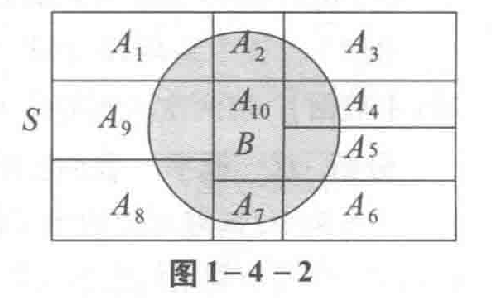
\includegraphics[scale=.5]{total_prob}
    \caption{全概公式示意图}
\end{figure}
\newpage
\qs{P14-10}{
    从1到9的整数中有放回地依次随机抽取3次,求取出的3个数之积能被10整除的概率.
}
显然这三个数中必有两数为$5$和$\{2,4,6,8\}$,因此
\pf{法一}{
    分情况讨论
    \begin{enumerate}
        \item A = \{三个数里有两个5和一个偶数\}
        \item B = \{三个数里有一个5和两个偶数\}
        \item C = \{三个数里有一个5一个偶数和一个其他的奇数\}
    \end{enumerate}
    那么有
    \(\Pr{A} = \frac{\binom{4}{1}\cdot 3}{9^3}\)\,\,%
    \(\Pr{B} = \frac{\binom{4}{1}\cdot 3+\tbinom{4}{2}\mathrm{A_3^3}}{9^3}\)\,\,%
    \(\Pr{C} = \frac{\binom{4}{1} \binom{4}{1} \mathrm{A_3^3}}{9^3}\)%
    相加得\(\frac{156}{729}\).
}
\pf{法二}{
    对立事件\\
    不妨设三个数中出现$5$的事件为$A$,出现偶数的事件为$B$,那么
    \begin{align*}
        \Pr{AB} & = 1 - \Pr{\overline{AB}}                                                                   \\
                & = 1 - \left(\Pr{\overline{A}} + \Pr{\overline{B}} - \Pr{\overline{A}\,\overline{B}}\right) \\
                & = 1- \left(\frac{8^3}{9^3} + \frac{5^3}{9^3} - \frac{4^3}{9^3}\right)                      \\
                & = \frac{156}{729}
    \end{align*}
}
\pf{法三}{
    另一种分情况讨论(笔者的分法)
    \begin{enumerate}
        \item A = \{三个数中有两个相同的\}
        \item B = \{三个数全不同\}
              \reversemarginpar\marginnote[\footnotesize\color{red}\textbf{此项须要分成下述两项,否则会重}]{}
              \begin{enumerate}[label*=\arabic*.]
                  \item$B_1$ = \{三个数全不同且有两个偶数\}
                  \item$B_2$ = \{三个数全不同且有两个奇数\}
              \end{enumerate}
    \end{enumerate}
    那么有
    \(\Pr{A} = \frac{\binom{4}{1}\binom{3}{1}+ \binom{4}{1}\binom{3}{1}}{9^3}\)\,\,%
    \(\Pr{B_1} = \frac{\binom{4}{1}\binom{4}{1}\binom{3}{1}}{9^3}\)\,\,%
    \(\Pr{B_2} = \frac{\binom{4}{1}\binom{4}{1}\mathrm{A_3^3}}{9^3}\)%
    相加得\(\frac{156}{729}\).
}
\nt{
    讨论各种情况的概率进而求得所求事件的概率的方法实际上是\vocab{全概率公式}的一种体现.
}
\subsection{Beyes公式}
\vocab{全概公式}是通过计算某一事件会发生的\textit{所有原因和情况的可能性大小}来计算该事件发生的概率,而\vocab{Beyes}公式则与之相反,考察一件已经发生的事情的\textit{各种原因或或情况的可能性大小}.
\thm{Beyes公式}{
    设$A_1,A_2,\cdots,A_n$是一个完备事件组,且$\Pr{A_i} >0\,\textrm{for i in 1\dots{n}}$,则对任一可能发生的事件$B$,有
    \begin{equation}
        \Pr{A_i|B}=\frac{\Pr{A_iB}}{\Pr{B}}=\frac{\Pr{A_i}\Pr{B|A_i}}{\sum_{j=1}^{n}\Pr{A_j}\Pr{B|A_j}}
    \end{equation}
}
\leftnote[-2.5cm]{$\Pr{A_i}$,$\Pr{A_i|B}$分别称为原因的\vocab{先验概率}和\vocab{后验概率}}
特别地,当$n=2$时,Beyes公式也可以写成
\begin{equation}
    \Pr{A|B}=\frac{\Pr{A}\Pr{B|A}}{\Pr{B}}
\end{equation}
\section{事件的独立性}
\leftnote[1cm]{\textbf{独立与互斥是两种不同的概念}}
\dfn{两事件独立性}{
    设$A,B$是两个事件,若
    \[\Pr{AB}=\Pr{A}\Pr{B}\]
    则称$A,B$\vocab{相互独立}.
}
\thm{}{
    设$A$,$B$两事件相互独立且$\Pr{B}>0$,则有
    \[\Pr{A|B}=\Pr{A}\]
}
\thm{}{
    若$A$,$B$两事件相互独立,则它们对立事件和其本身(不同事件间)的组合也相互独立.
}

根据三个事件(略)独立性的定义,可以类推到n个事件的独立性:
设$A_1,A_2,\cdots,A_n$是$n$个事件,若对于其中任意$k(2\leq k\leq n)$个事件$A_{i_1},A_{i_2},\cdots,A_{i_k}$,有
\begin{equation}
    \Pr{A_{i_1}A_{i_2}\cdots A_{i_k}}=\Pr{A_{i_1}}\Pr{A_{i_2}}\cdots\Pr{A_{i_k}}
\end{equation}
则称$A_1,A_2,\cdots,A_n$\vocab{相互独立}.
\dfn{}{
    设$A_1,A_2,\cdots,A_n\,(n > 2)$是$n$个事件,若其中任意两个事件相互独立,则称这$n$个事件\vocab{两两独立}.
}
由此可以得到多个独立事件所具备的性质
\cor{}{
    设$A_1,A_2,\cdots,A_n\,(n > 2)$相互独立,则其中任意$k(2\leq k\leq n)$个(它们的对立)事件也相互独立.
}
\section{Bernoulli试验}
即两点分布.
\leftnote[1.8cm]{这相当于在实验结果序列中任取k次发生A事件}
\thm{Bernoulli定理}{
    一次试验中,事件$A$发生的概率为$p$,进行这样的试验n次,事件$A$发生$k$次的概率为
    \[b(k;n;p) = \binom{n}{k}p^k(1-p)^{n-k}\]
}
\nt{
n次Bernoulli试验的概率分布就是二项分布.其概率密度函数为
\[f(k,n,p)=\Pr(k;n,p)=\Pr(X=k)={\binom {n}{k}}p^{k}(1-p)^{n-k}\]
\textbf{Glossary}:两点分布=Bernoulli试验;二项分布=多次Bernoulli试验=Bernoulli概型.
}
\pf{辨析}{
    $\Pr{A}$ 和$\Pr(X)$使用的括号不同.大括号代表是事件,即一系列样本点集合(故而用大括号),小括号代表是随机变量(因为此时是概率密度函数).
}
\chapter{随机变量及其分布}
\section{随机变量}
\dfn{随机变量}{
    设随机试验的样本空间为$S$, 称定义在$S$上的实值单值函数$X=X(\omega)$为\vocab{随机变量}.\\
    亦即
    \[X:\omega\mapsto x_i \in \RR\, \, \ie\, \, S\rightarrow\RR\]
}
实际上, $\Pr(X=a)$是$A=\{\omega|X(\omega)=a\}$的简记.
\section{离散型随机变量及其分布}
设$X$是一个随机变量, 如果$X$的所有可能取值为有限个或可列无限多个, 则称$X$为\vocab{离散型随机变量}.
\dfn{离散型随机变量分布律}{
    设$X$是一个离散型随机变量, 如果
    \[\Pr(X=x_k)=p_k, k=1, 2, \ldots\]
    则称$p_k$为$X$的\vocab{分布律}或\vocab{概率分布}, 亦称\vocab{概率质量函数} (PMF). 记为$f_X(x)$.
}
就是高中所学之分布列.
\subsection{常用离散分布}
\subsubsection{两点分布}
\dfn{两点分布}{
    设$X$的分布律为
    \begin{align}
        \Pr(X=k)=\begin{cases}
                     p,   & k=x_1 \\
                     1-p, & k=x_2
                 \end{cases}
    \end{align}

    其中$0<p<1$, 则称$X$服从以$p$为参数的\vocab{两点分布}.
}
若$X$服从$x_1 = 1, x_2 = 0$处参数为$p$的两点分布, 则称其服从参数为$p$的\vocab{0-1分布}.
\newpage
\subsubsection{二项分布}
\leftnote[1cm]{当$n=1$时, 二项分布退化为0-1分布.}
\dfn{二项分布}{
    设$X$的分布律为
    \begin{equation}
        \Pr(X=k)=\binom{n}{k}p^k(1-p)^{n-k}, \, \, k=0, 1, \ldots, n
    \end{equation}
    其中$n$为正整数, $0<p<1$, 则称$X$服从参数为$n, p$的\vocab{二项分布}, 记为$X\sim B(n, p)$.
}
\leftnote{$\sim$记号就是\textbf{服从}的意思}
二项概率总存在一个最大值$M$ \st \((n+1)p-1\leq M<(n+1)p\).
\subsubsection{Poisson分布}
\dfn{Poisson分布}{
    设$X$的分布律为
    \begin{equation}
        \Pr(X=k)=\frac{\lambda^k}{k!}e^{-\lambda}, \, \, k=0, 1, \ldots
    \end{equation}
    其中$\lambda>0$, 则称$X$服从参数为$\lambda$的\vocab{Poisson分布}, 记为$X\sim P(\lambda)$.
}
因为$e^x=1+\sum_{n=1}^{\infty}\frac{x^n}{n!}$, 将$x$换为$\lambda$可得泊松分布的概率和为1.
\section{累积分布函数}
\subsection{随机变量的分布函数}
\dfn{随机变量CDF}{
    设$X$是一个随机变量, 对任意实数$x$, 定义
    \[F(x)\defeq\Pr(X\leq x)\in [0, 1]\]
    称$F(x)$为$X$的\vocab{累积分布函数}(CDF). 有时记作$F_X(x)$或$X\sim F(x)$.
}
分布函数$F(x)$的值就表示$X$落在区间$(-\infty, x]$的概率.
\subsubsection{性质}
\begin{enumerate}
    \item \textit{单调非减性}: $x_1<x_2\Rightarrow F(x_1)\leq F(x_2)$
    \item $F(-\infty) = \lim_{x\rightarrow -\infty}F(x) = 0, \, \, F(+\infty) = \lim_{x\rightarrow +\infty}F(x) = 1$.
    \item \textit{右连续性}: $\lim_{x\rightarrow x_0^+}F(x) = F(x_0)$
\end{enumerate}
具有上述性质的函数一定是某个随机变量的CDF.
\newpage
\subsection{离散型随机变量的分布函数}
\begin{wrapfigure}[10]{r}{.3\textwidth}
    \centering
    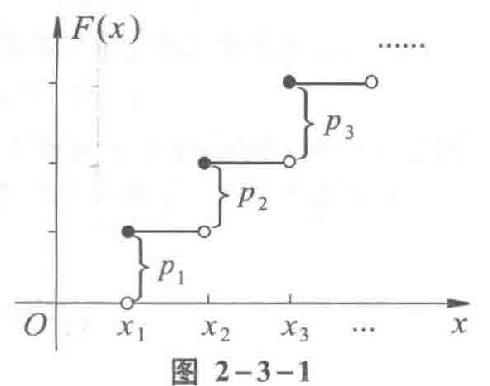
\includegraphics[scale=.5]{cdf_discrete}
    \caption{阶梯型CDF}
\end{wrapfigure}
在上述基础上, 对于离散型随机变量$X$有CDF:
\[F(x) = \Pr(X\leq X) = \sum_{x_i\leq x}\Pr(X=x_i)\]
$F(x)$是一个\vocab{阶梯型函数}, 在点$x_i$处的跃度为$\Pr(X=x)$.
可以看出阶梯型函数符合CDF之性质:总是右连续的;而作为一个分段函数来说, 其各段区间总是(习惯上)左闭右开的.
\nt{
    考题中由CDF反推分布列可以根据每一个左侧端点得到对应的随机变量$x_i$.\\
    计算分布列时, 有公式$\Pr{a\leq X< b} = F(b) - F(a)$.
}
随机变量$X$的CDF为阶梯型函数$\Leftrightarrow$ $X$是离散型随机变量.
\section{连续型随机变量及其概率密度}
\dfn{PDF}{
    设$X$是一个随机变量, 如果存在非负可积函数$f(x)$, 使对任意实数$x$有
    \begin{equation}
        F(x) =  \Pr{X\leq x} = \int_{-\infty}^xf(t)\dd{t}
    \end{equation}
    则称$X$为\vocab{连续型随机变量}, $f(x)$为$X$的\vocab{概率密度函数}(PDF).
}
立即可以得到PDF的性质
\begin{enumerate}
    \item $f(x)\geq 0$;
    \item $\int_{-\infty}^{+\infty}f(x)\dd{x} = 1$.
    \item $F'(x) = f(x)$. 若$f(x)$在$x$处连续
\end{enumerate}
\nt{
    若某个随机变量的CDF可以写成PDF积分函数的形式, 则称其为连续型随机变量.
}
\pf{证明\quad $X$取任一特值的概率为$0$}{
    \begin{align*}
        \mbox{考虑极限}
        \Pr{X=a} & =\lim_{\Delta x \to 0^+}\Pr{a-\Delta x \le X \leq a}    \\
        \mbox{对RHS积分, 有}                                                   \\
        \Pr{X=a} & =\lim_{\Delta x \to 0^+}\int_{a-\Delta x}^{a}f(x)\dd{x} \\
                 & =0.
    \end{align*}
}
由上面的证明我们可以知道以下的性质
\begin{equation}
    \Pr{a< X< b } = F(b ) - F(a ) = \int_{a }^{b }f(x )\dd{x}.
\end{equation}
这个等式无论X两侧端点开闭都成立.
\subsection{常用连续型分布}
\subsubsection{均匀分布}
\dfn{均匀分布}{
    设$X$的概率密度为
    \begin{equation}
        f(x)=\begin{cases}
            \frac{1}{b-a}, & a<x<b     \\
            0,             & otherwise
        \end{cases}
    \end{equation}

    其中$a<b$, 则称$X$服从参数为$a, b$的\vocab{均匀分布}, 记为$X\sim U(a, b)$.
}
\leftnote[-1cm]{U for Uniform}
设$[a, b]$之间的任意子区间为$[c, d]$, 由上式可得$\Pr{c<X<d}=\int_{c }^{d }\frac{1}{b-a}\dd{x} = \frac{d-c}{b-a}$.\\因而我们可以得到
\begin{equation}
    F(x) = \begin{cases}
        0,               & x < a     \\
        \frac{x-a}{b-a}, & a\leq x<b \\
        1,               & x\geq b
    \end{cases}
\end{equation}
\subsubsection{指数分布}
\dfn{指数分布}{
    若随机变量$X$的概率密度为
    \begin{equation}
        f(x)=\begin{cases}
            \lambda e^{-\lambda x}, & x>0     \\
            0,                      & x\leq 0
        \end{cases}, \lambda > 0
    \end{equation}
    则称X服从参数为$\lambda$ 的\vocab{指数分布}, 记为$X\sim E(\lambda)$.
}
积分得
\begin{equation}
    F(x)=\begin{cases}
        1-e^{-\lambda x}, & x>0     \\
        0,                & x\leq 0
    \end{cases}
\end{equation}
\subsubsection{正态分布}
\dfn{正态分布}{
    若随机变量$X$的概率密度为
    \begin{equation}
        f(x)=\frac{1}{\sqrt{2\pi}\sigma}e^{-\frac{(x-\mu)^2}{2\sigma^2}}, \, \, \left(-\infty<x<+\infty\right)
    \end{equation}
    其中$\mu, \sigma(\sigma>0)$为常数, 则称$X$服从参数为$\mu, \sigma^2$的\vocab{正态分布}, 记为$X\sim N(\mu, \sigma^2)$.
}
\qs{Poisson积分}{
\textbf{不使用Wallis公式}, 求Poisson积分\;$\displaystyle\int_{-\infty}^{+\infty}e^{-t^2}\dd{t}$.
}
\sol{
    \textit{转化为求累次积分}
    \begin{align}
        \intertext{要求原式, 不妨先求其平方, 亦即}
        \left(\int_{-\infty}^{+\infty}e^{-t^2}\dd{t}\right)^2 & = \int_{-\infty}^{+\infty}e^{-x^2}\dd{x}\int_{-\infty}^{+\infty}e^{-y^2}\dd{y} \nonumber \\
        \intertext{化为累次积分有}
                                                              & = \iint_{\RR[2]}e^{-(x^2+y^2)}\dd{x}\dd{y}.  \nonumber                                   \\
        \intertext{$\RR[2]$即$xOy$面, 化为极坐标有}
        \iint_{\RR[2]}e^{-\rho^2}\rho\dd{\rho}\dd{\theta}     & = \int_{0}^{2\pi}\dd{\theta}\int_{0}^{+\infty}e^{-\rho^2}\rho\dd{\rho}       \nonumber   \\
                                                              & = \pi                                                                         \nonumber  \\
        \tf \int_{-\infty}^{+\infty}e^{-t^2}\dd{t}            & = \sqrt{\pi}.
    \end{align}
}
通过计算Poisson积分, 我们可以得到正态分布的PDF重要性质:
\begin{equation}
    \int_{-\infty}^{+\infty}\frac{1}{\sqrt{2\pi}\sigma}e^{-\frac{(x-\mu)^2}{2\sigma^2}}\dd{x} = 1
\end{equation}
\textbf{图形特征}
\begin{figure}[h]
    \centering
    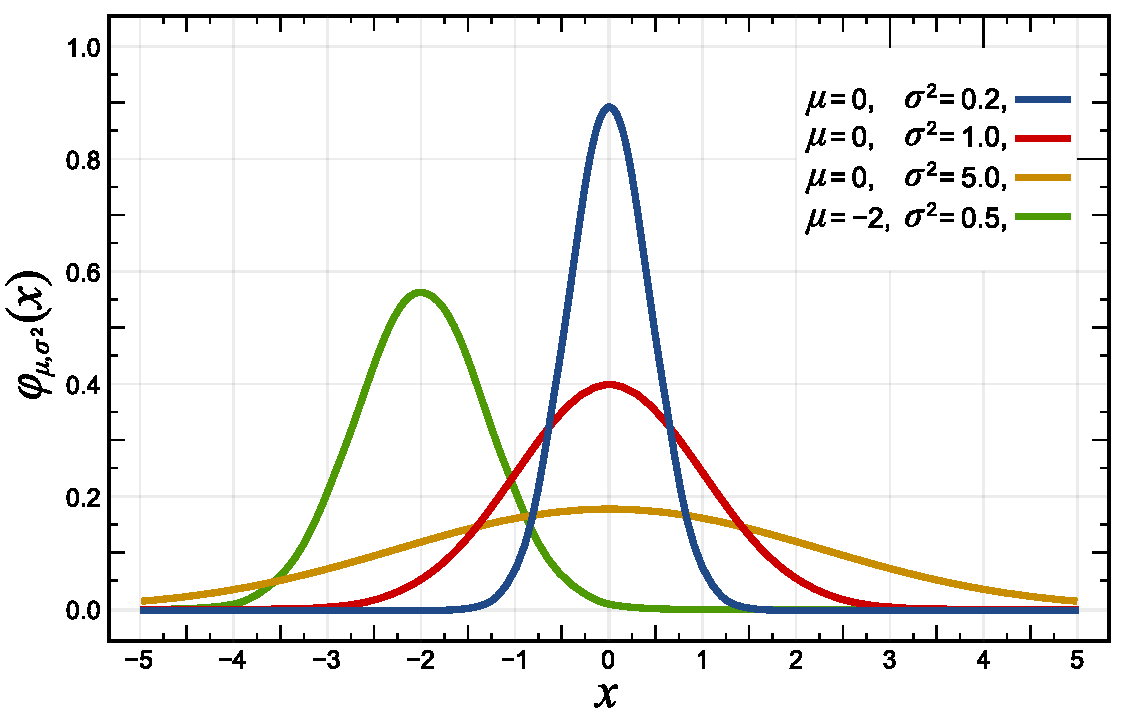
\includegraphics[scale=.7]{Normal_Distribution_PDF}
    \caption{PDF}
\end{figure}
\leftnote[4.8cm]{$\sigma$越小, 方差越大, 曲线中峰越陡}
\begin{enumerate}
    \item $\mu$确定曲线位置, $\sigma$确定曲线中峰的陡峭程度
    \item 密度曲线关于$x=\mu$对称
    \item 密度曲线在$x=\mu$处有最大值$\frac{1}{\sqrt{2\pi}\sigma}$
    \item 密度曲线在$x=\mu\pm\sigma$处有拐点且以$x$轴为渐近线
\end{enumerate}
当$\mu=0, \sigma=1$时, 称为\vocab{标准正态分布}, 记为$X\sim N(0, 1)$, PDF用$\phi(x )$表示, CDF用$\Phi(x )$表示:
\leftnote[1.1cm]{\textbf{\color{red}显然$\phi(x)$为偶函数.}}
\begin{align}
    \phi(x ) = \frac{1}{\sqrt{2\pi}}e^{-\frac{x^2}{2}} &  & \Phi(x ) = \int_{-\infty}^{x}\phi(t)\dd{t}
    \label{eq:2.13}
\end{align}
\thm{重要定理}{
    设$X\sim N(\mu, \sigma^2)$, 则$Y= \frac{X-\mu}{\sigma}\sim N(0, 1)$.\\
    计算$\Pr{Y\leq x}$时, 可转化为计算$\Pr{X\leq \mu + \sigma x}$, 计算此时的$\Phi(x)$即得证.
}
这说明任意一般的正态分布都可以通过\textbf{线性变换}转化为标准正态分布.
因此X的分布函数也可以写成
\[F(x) = \Phi\left(\frac{x-\mu}{\sigma}\right)\]
\[\Pr{a<X<b}= \Pr{\frac{a-\mu}{\sigma}<Y<\frac{b-\mu}{\sigma}} = \Phi\left(\frac{b-\mu}{\sigma}\right) - \Phi\left(\frac{a-\mu}{\sigma}\right)\]
\section{随机变量函数的分布}
前面提到计算$\Pr{Y\leq x}$时, 可转化为计算$\Pr{X\leq \mu + \sigma x}$, 其中的$Y=\frac{X-\mu}{\sigma}$是随机变量$X$的函数, 因此$Y$也是随机变量.
\dfn{随机变量函数}{
    若存在一个函数$g(x)$ s.t. 随机变量$X, Y$满足
    \begin{equation*}
        Y=g(X)
    \end{equation*}
    称$Y$为$X$的一个\vocab{随机变量函数}.
}
\subsection{离散型随机变量函数的分布}
根据上述定义, 显然$X$的函数$Y$也是一个随机变量.
\subsubsection{导出$Y$的分布律}
首先确定$Y$的所有取值, 通过$Y$的每一个值$y_i\, (i=1, 2, \ldots)$确定相应的\\
(注:我们用$C_i$来表示$X$的取值为$x_i$时, 与对应$Y$匹配的$X$的取值的集合)
\begin{equation*}
    C_i=\{x_i | g(x_j) = y_i\},
\end{equation*}
\begin{equation*}
    \{Y=y_i\}=\{X\in C_i\},
\end{equation*}
那么有\\
\begin{equation}
    \Pr{Y=y_i} = \Pr{X\in C_i } = \sum_{x_j \in C_i }\Pr{X=x_j} \label{eq:2.14}
\end{equation}
为Y的分布律.这表明: \textbf{$Y$的分布律完全由$X$的分布律确定}.
\subsection{连续型随机变量函数的分布}
\leftnote{分布律:离散变量\\PDF: 连续变量}
通过上述定义, 不难发现连续随机变量的函数\textit{不一定}是连续型随机变量.
\nt{
    考虑\emph{符号函数}作为映射法则:
    \begin{equation*}
        Y = \sign(x) = \begin{cases}
            1, & x>0  \\
            0, & x= 0 \\
            -1 & x<0
        \end{cases}
    \end{equation*}
    显然$Y=0, \pm 1$, 是一个离散型随机变量.因此, 在连续型的情况下, $Y$的连续性由其自身决定.
}
\subsubsection{导出$Y$的PDF}
已知$X$的CDF\, $F_X(x )$或PDF\, $f_X(x )$, 则$Y=g(x )$的CDF可以通过以下公式求得:
\begin{equation}
    \begin{split}
        F_Y(y ) = \Pr{Y\leq y } = \Pr{g(X)\leq y } = \Pr{X\in C_y }, \, \mbox{其中}\, C_y = \{x | g(x )\leq y \}.
    \end{split}
\end{equation}
之后通过积分$\int_{C_y }f_X(x )\dd{x}$求得CDF.
\exc{离散变量函数导出PMF}{
    给出随机变量$X$的分布律如下, 试求$Y=X^2$的分布律:
    \begin{center}
        \begin{tabular}{@{}cccccc@{}}
            \toprule
            $X$   & $-2$  & $-1$  & $0$   & $1$    & $3$     \\ \midrule
            $p_i$ & $1/5$ & $1/6$ & $1/5$ & $1/15$ & $11/30$ \\ \bottomrule
        \end{tabular}
    \end{center}
}
\sol{
    由题意得$Y=0, 1, 4, 9, $, 因此利用\eqref{eq:2.14}计算得
    \begin{align*}
        \Pr{Y=0} = \Pr{X=0} = \frac{1}{5} &  & \Pr{Y=1} = \Pr{X=\pm 1} = \frac{7}{30} \\
        \Pr{Y=4} = \Pr{X=-2}= \frac{1}{5} &  & \Pr{Y=9} = \Pr{X=3} = \frac{11}{30}
    \end{align*}
    \begin{center}
        $\tf$\;
        \begin{tabular}{@{}ccccc@{}}
            \toprule
            $Y$   & $0$   & $1$    & $4$   & $9$     \\ \midrule
            $p_i$ & $1/5$ & $7/30$ & $1/5$ & $11/30$ \\ \bottomrule
        \end{tabular}
    \end{center}
}
\exc{连续变量函数导出PDF}{
    设$X$服从\textit{标准正态分布}, 求$Y=2X^2+1$的PDF
}
\sol{
    要求PDF, 不妨先求Y的CDF $F_Y(y )$ \ie $\Pr{Y\leq y }$, 代入有
    \begin{align*}
        F_Y(y ) = \Pr{2X^2 +1 \leq y} & = \Pr{\sqrt{-\frac{y-1}{2}}\leq X \leq \sqrt{\frac{y-1}{2}}}                                                                                                                                                       \\
                                      & =\begin{cases*}
                                             {\displaystyle\int_{-\sqrt{\frac{y-1}{2}}}^{\sqrt{\frac{y-1}{2}}}f_X(x )\dd{x}} & $y> 1$    \\
                                             0                                                                               & otherwise
                                         \end{cases*}                                                                                                                       \\
                                      & = \begin{cases*}
                                              F_X\left(\sqrt{\frac{y-1}{2}}\right) - F_X\left(-\sqrt{\frac{y-1}{2}}\right) & $y> 1$    \\
                                              0                                                                            & otherwise
                                          \end{cases*}
    \end{align*}
    \begin{align*}
        \tf\; f_Y(y ) = F_Y'(y) = \begin{cases*}
                                      {\displaystyle\sqrt{2}\, \frac{\color{red}f_X\left(\sqrt{\frac{y-1}{2}}\right)}{4\sqrt{y-1}} + \sqrt{2}\, \frac{\color{red}f_X\left(-\sqrt{\frac{y-1}{2}}\right)}{4\sqrt{y-1}}} & $y > 1$   \\
                                      0                                                                                                                                                                               & otherwise
                                  \end{cases*}
    \end{align*}
    \begin{equation*}
        \tf\quad\phi(x ) = \frac{1}{\sqrt{2\pi}}e^{-\frac{x^2}{2}}\;\eqref{eq:2.14}\quad\text{注意到$\phi(x)$为偶函数, 合并上述\color{red}两项}
    \end{equation*}
    \begin{align*}
        \Longrightarrow f_Y(y ) = \begin{cases*}
                                      \frac{1}{2\sqrt{\pi (y-1)}}e^{-\frac{y-1}{4}} & $y> 1$    \\
                                      0                                             & otherwise
                                  \end{cases*}
    \end{align*}
}
\chapter{多维随机变量及其分布}
\section{二维随机变量及其分布}
\subsection{二维随机变量}
\dfn{二维随机变量}{
    设随机试验的样本空间为$S$,定义在$S$上的实值单值函数$X = X(\omega)\;Y=Y(\omega)$为两个随机变量.称向量$(X,Y )$为定义在$S$上的\vocab{二维随机变量}
    \begin{center}
        \ie    $\begin{aligned}
                X:S     & \to\RR                                              \\
                Y:S     & \to\RR                                              \\
                (X,Y):S & \to\RR[2]\;\ie\;\omega\mapsto (X(\omega),Y(\omega))
            \end{aligned}$
    \end{center}
}
类似地,我们可以得到$n$维随机变量的定义.
\subsection{二维随机变量的分布函数}
\dfn{二维随机变量的分布函数}{
    设$(X,Y)$是二维随机变量,对于任意实数$x,y$,定义二元函数
    \begin{equation}
        F(x,y) = \Pr{X\leq x\cap Y\leq y} \defeq \Pr{X\leq x, Y\leq y}
    \end{equation}
    称为二维随机变量$(X,Y)$的\vocab{分布函数},或\vocab{联合分布函数(Joint CDF)}.
}
\begin{figure}[h]
    \centering
    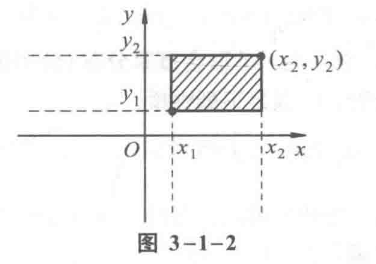
\includegraphics[scale=.8]{jointCDF}
    \caption{CDF}
\end{figure}
将这个向量视作平面内随机点的坐标,分布函数就是随机点$(X,Y)$落入矩形域的概率.通过容斥原理计算得到
\begin{equation}
    \Pr{x_1\leq X \leq x_2, y_1\leq Y\leq y_2} = F(x_2,y_2) - F(x_1,y_2) - F(x_2,y_1) + F(x_1,y_1)
\end{equation}
\newpage
\subsubsection{联合CDF的性质}
\leftnote[1cm]{右侧几个等式可通过矩形域的面积来理解.}
\begin{enumerate}
    \item $0\leq F(x,y )\leq 1$
          \begin{enumerate}
              \item 固定$y$,$F(-\infty,y ) = 0$;
              \item 固定$x$,$F(x,-\infty) = 0$;
              \item $\lim_{\substack{x\to +\infty\\y\to +\infty}}F(x,y ) = 1, \lim_{\substack{x\to -\infty\\y\to -\infty}}F(x,y) = 0$
          \end{enumerate}
    \item (\emph{单调性})$F(x,y )$关于$x$和$y$都是单调不减的.
          \begin{enumerate}
              \item 固定$y$,$F(x,y )$关于$x$单调不减;
              \item 固定$x$,$F(x,y )$关于$y$单调不减.
          \end{enumerate}
    \item (\emph{连续性})$F(x,y )$关于$x$和$y$都是右连续的.
\end{enumerate}
若已知$(X,Y)$的分布函数$F(X,Y)$,则可由之导出各个参数(在固定另一个参数的情况下)各自的分布函数:
\begin{align}
    F_X(X) & = \Pr{X\leq x } =\Pr{X\leq x} = \lim_{y\to +\infty}F(x,y), \\
    F_Y(y) & = \Pr{Y\leq y } =\Pr{Y\leq y} = \lim_{x\to +\infty}F(x,y),
\end{align}
如此导出的CDF称为\vocab{边缘分布函数}.
\subsection{二维离散型随机变量及其分布律}
\dfn{联合概率分布律}{
    设$(X,Y)$是二维离散型随机变量,若存在非负函数$p_{ij}$,使得
    \begin{equation}
        \Pr{X=x_i,Y=y_j} = p_{ij},\quad i,j=1,2,\cdots
    \end{equation}
    则称$(X,Y)$为二维离散型随机变量,并称$p_{ij}$为$(X,Y)$的\vocab{联合概率分布律}.
}
显然,$p_{ij}$满足性质:\;\;
\begin{enumerate*}
    \item $p_{ij}\geq 0$;
          \quad\item $\sum_i\sum_j p_{ij} = 1$.
\end{enumerate*}
利用其分布律,易见$(X,Y )$在$D$上的概率为
\begin{equation}
    \Pr{(X,Y)\in D} = \sum_{(x_i,y_j)\in D}p_{ij}
\end{equation}
而其联合CDF为
\begin{equation}
    F(x,y) = \Pr{X\leq x, Y\leq y } = \sum_{x_i\leq x,\,y_j\leq y}p_{ij}
\end{equation}
\subsubsection{边缘分布律}
通过联合概率分布,我们可以得到$X,Y$各自的概率分布:
\leftnote[.5cm]{即行和,列和}
\begin{align}
    p_{i\cdot}  & = \Pr{X=x_i} = \sum_j p_{ij} \\
    p_{\cdot j} & = \Pr{Y=y_j} = \sum_i p_{ij}
\end{align}
这称为$(X,Y)$的\vocab{边缘分布}.
\qs{例1}{设随机整数变量$X=1,2,3,4$,$Y=1\cdots X$等可能地取值,试求$(X,Y)$的分布律.}
\sol{
    \begin{align*}
        \mbox{由题意可得}\Pr{X=i,Y=j} & = \Pr{Y=j|X=i}\Pr{X=i}\eqref{eq:mul}                   \\
                                 & = \frac{1}{i }\cdot\frac{1 }{4 }, i =1,2,3,4, j\leq i.
    \end{align*}
    \begin{center}
        \begin{tabular}{@{}ccccc@{}}
            \toprule
            $X,Y$ & $1$    & $2$    & $3$    & $4$    \\ \midrule
            $1$   & $1/4$  & $0$    & $0$    & $0$    \\ \midrule
            $2$   & $1/8$  & $1/8$  & $0$    & $0$    \\ \midrule
            $3$   & $1/12$ & $1/12$ & $1/12$ & $0$    \\ \midrule
            $4$   & $1/16$ & $1/16$ & $1/16$ & $1/16$ \\ \bottomrule
        \end{tabular}
    \end{center}
}
\subsection{二维连续型随机变量及其概率密度}
\dfn{二维连续型随机变量}{
    设$(X,Y)$是二维随机变量,$F(X,Y)$为其分布函数,若存在非负可积函数$f(x,y)$ s.t.
    \begin{equation*}
        F(x,y) = \int_{-\infty}^x\int_{-\infty}^y f(u,v)\dd{u}\dd{v}
    \end{equation*}
    则称$(X,Y)$为\vocab{二维连续型随机变量},称$f(x,y)$为其\vocab{概率密度}
}
显然,$f(x,y)$满足性质:\;\;
\begin{enumerate*}[label=\bfseries\protect\circled{\arabic*}]
    \item $f(x,y)\geq 0$;\quad
    \item $\int_{-\infty}^{+\infty}\int_{-\infty}^{+\infty}f(x,y)\dd{x}\dd{y} =F(+\infty,+\infty)=1$.
\end{enumerate*}

\textbf{重要性质}\quad 设$D$是$xOy$平面上的区域,$(X,Y )$落入其中的概率为
\begin{equation}
    \Pr{(X,Y)\in D} = \iint_D f(x,y)\dd{x}\dd{y}
\end{equation}
若$f(x,y)$在$(x,y )$处连续,则有
\begin{equation}
    \pdv{F(x,y)}{x}{y} = f(x,y).
\end{equation}
\subsubsection{边缘概率密度}\label{sec:marginPDF}
我们知道此处的$X$和$Y$都是都是连续型随机变量,可得它们的\vocab{边缘密度}为
\begin{align}
    f_X(x)=\int_{-\infty}^{+\infty}f(x,y )\dd{y}; &  & f_Y(y)=\int_{-\infty}^{+\infty}f(x,y )\dd{x};
    \label{eq:3.12}
\end{align}
结合之前的性质,我们可以知道对$F(x,y)$求一个变量的偏导可以得到另一个变量的边缘密度.
\leftnote[2cm]{通常都是分段函数,且一段为$0$\\(\emph{不然很难算})}
\exc{习题3-1-6改}{
    设随机变量$(X,Y )$的概率密度为
    \begin{align*}
        f(x,y) = \begin{cases}
                     k(6-x-y), & 0<x<2, 2<y<4 \\
                     0,        & \mbox{else}
                 \end{cases}
    \end{align*}
    求\begin{enumerate*}[label=\bfseries\protect\circled{\arabic*}]
        \item 常数$k$;\;\;
        \item $\Pr{X+Y \leq 4}$;\;\;
        \item $X,Y$的边缘密度.
    \end{enumerate*}
}
\sol{
(1)因为

\begin{align*}
    \iint_{\RR[2]}f(x,y)\dd{x}\dd{y} =\begin{cases}
                                          \iint_Dk(6-x-y)\dd{x}\dd{y}, & x\in D=\{(x,y)|x\in (0,2) y\in (2,4)\} \\
                                          0,                           & \mbox{else}
                                      \end{cases} =1
\end{align*}
\[\ie \iint_Dk(6-x-y )\dd{x}\dd{y} = \int_{0}^{2}\int_{2}^{4}k(6-x-y )\dd{x}\dd{y} = 1,\mbox{计算得}k = \frac{1}{8}.\]
\newpage
\noindent (2)由题意,所有符合的$(X,Y)$至少落在直线$x + y = 4$的左侧.由(1)知点只可能落入$D$中,故令\\$G = D\cap \{x+y\leq 4\}$,即下图{\color[HTML]{8e3a16}\emph{棕色区域}}
    \leftnote[1.8cm]{w/ Geogebra}
    \begin{center}
        \usetikzlibrary{arrows}
\definecolor{zzttqq}{rgb}{0.6,0.2,0}
\definecolor{xdxdff}{rgb}{0.49019607843137253,0.49019607843137253,1}
\definecolor{uuuuuu}{rgb}{0.26666666666666666,0.26666666666666666,0.26666666666666666}
\begin{tikzpicture}[line cap=round,line join=round,>=triangle 45,x=1cm,y=1cm,scale=.6,thick]
    \begin{axis}[
            x=1cm,y=1cm,
            axis lines=middle,
            xmin=-1.0430999574123194,
            xmax=4.793645986891604,
            ymin=-0.3419648743673125,
            ymax=4.411066384011339,
            xtick={-1,0,...,4},
            ytick={0,1,...,4},]
        \clip(-1.0430999574123194,-0.3419648743673125) rectangle (4.793645986891604,4.411066384011339);
        \fill[line width=2pt,color=zzttqq,fill=zzttqq,fill opacity=0.10000000149011612] (0,4) -- (0,2) -- (2,2) -- cycle;
        \draw [line width=2pt,domain=-1.0430999574123194:4.793645986891604] plot(\x,{(--4-1*\x)/1});
        \draw [line width=2pt,color=zzttqq] (0,4)-- (0,2);
        \draw [line width=2pt,color=zzttqq] (0,2)-- (2,2);
        \draw [line width=2pt,color=zzttqq] (2,2)-- (0,4);
        \begin{scriptsize}
            \draw[color=black] (0.5,4.184310865488937) node {$eq1$};
            \draw [fill=uuuuuu] (0,4) circle (2pt);
            \draw [fill=xdxdff] (0,2) circle (2.5pt);
            \draw [fill=xdxdff] (2,2) circle (2.5pt);
        \end{scriptsize}
    \end{axis}
\end{tikzpicture}
    \end{center}
    那么,我们有
    \[k\cdot\iint_G6-x-y \dd{x}\dd{y} = \Pr{X+Y\leq 4}= \frac{2}{3}\;\;\mbox{即为所求}.\]
    \leftnote[2cm]{相当于固定一个变量,对另一个变量积分}
    (3)根据\ref{sec:marginPDF},可以得到
    \begin{align*}
        f_X(x) & = \begin{cases}
                       {\displaystyle\frac{1}{8}\cdot\int_{2}^{4-x}(6-x-y)\dd{y} = \frac{1}{8}(6-4x+\frac{1}{2}x^2)}, & 0<x<2       \\
                       0,                                                                                             & \mbox{else}
                   \end{cases}                                          \\
               & \mbox{同理可得}                                                                                                                                                               \\
        f_Y(y) & = \begin{cases}
                       {\displaystyle\frac{1}{8}\cdot\int_{0}^{4-y}(6-x-y)\dd{x} = \mbox{(\dots\;略)}},\hphantom{(4x+\frac{1}{2}x^2)} & 2<y<4       \\
                       0,                                                                                                            & \mbox{else}
                   \end{cases}
    \end{align*}
    }
    \subsection{二维均匀分布}
    \dfn{二维均匀分布}{
        设$G$是平面上的有界区域,其面积为$A$,若二维随机变量$(X,Y )$具有概率密度函数
        \begin{align}
            f(x,y)=\begin{cases}
                       \frac{1}{A}, & (x,y)\in G  \\
                       0,           & \mbox{else}
                   \end{cases}
        \end{align}
        则称$(X,Y )$在$G$上服从\vocab{二维均匀分布}.
    }
    \begin{wrapfigure}[4]{r}{95pt}
        \begin{center}
            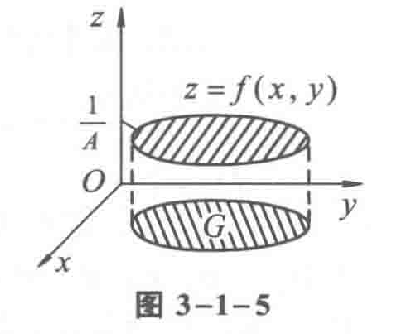
\includegraphics[scale=.5]{2dUniform}
        \end{center}
        \caption{均匀分布}
    \end{wrapfigure}
    若$(X,Y)$在$G$上服从均匀分布,则其概率密度函数反映在几何上为定义在$xOy$平面内区域$G$上的空间的一块平面.
    考虑向平面$G$上投掷一质点,若点落在区域$B\subseteq G$内的概率与$B$的面积成正比且与$B$的位置无关,则称$G$为均匀分布的区域,
    坐标$(X,Y)$在$G$上服从均匀分布.
    \leftnote[2.5cm]{\color{red}对于\textbf{矩形域}$G$该公式成立,其他形状则不一定.}
    \cor{}{
        均匀分布$(X,Y)$的两个边缘分布仍为均匀分布且分别为
        \begin{align}
            \begin{split}
                f_X(x) & = \begin{cases}
                               \frac{1}{b-a}, & a<x<b       \\
                               0,             & \mbox{else}
                           \end{cases} \\
                f_Y(y) & = \begin{cases}
                               \frac{1}{d-c}, & c<y<d       \\
                               0,             & \mbox{else}
                           \end{cases}
            \end{split}
        \end{align}
    }

    \qs{例5}{
        设$(X,Y)$服从\emph{单位圆域}上的均匀分布,求对应的两个边缘分布.
    }
    \newpage
    \sol{
        由题意得,其PDF为
        \begin{align*}
            f(x,y) & = \begin{cases}
                           \frac{1}{\pi}, & x^2+y^2\leq 1 \\
                           0,             & \mbox{else}
                       \end{cases}
        \end{align*}
        根据\eqref{eq:3.12},只需考虑点在圆域内的情况,易得
        \begin{align*}
            f_X(x)     & = \frac{1}{\pi}\int_{-\sqrt{1-x^2}}^{\sqrt{1-x^2}}\dd{y} = \frac{2}{\pi}\sqrt{1-x^2}. \\
            \tf f_X(x) & = \begin{cases}
                               \frac{2}{\pi}\sqrt{1-x^2}, & -1\leq x\leq 1 \\
                               0,                         & \mbox{else}
                           \end{cases}
        \end{align*}
        因为$x^2 + y^2 \leq 1$是\emph{轮换式},将$x$换成$y$即可得到$f_Y(y)$.
    }
    \section{随机变量的独立性}
    \dfn{独立性}{
        设$(X,Y)$是二维随机变量,若对于任意$x,y$,
        \begin{align}
            \begin{split}
                \Pr{X\leq x, Y\leq y} & = \Pr{X\leq x}\Pr{Y\leq y} \\
                \ie\;F(x,y)           & = F_X(x)F_Y(y) \text{充要条件}
                \label{eq:3.15}
            \end{split}
        \end{align}
        则称$X$和$Y$是\vocab{相互独立}的.
    }
    \thm{}{
        随机变量$X,Y$相互独立的充要条件是对$X$和$Y$所生成的任何事件相互独立,即
        \begin{equation}
            \Pr{X\in A, Y\in B} = \Pr{X\in A}\Pr{Y\in B}
        \end{equation}
    }
    \subsection{离散型随机变量的独立性}
    若$X,Y$是离散型随机变量,可以由此判断其独立性:\\
    \textbf{定义2}\quad 若对$(X,Y)$的所有可能取值$(X_i,Y_i)$有
    \begin{align}
        \Pr{X=X_i,Y=Y_j} & = \Pr{X=X_i}\Pr{Y=Y_j},\nonumber \\
        \ie\;p_{ij}      & = p_{i\cdot}p_{\cdot j}
    \end{align}
    则称$X,Y$相互独立.
    \exc{P\textsubscript{77}11}{
        设$X,Y$相互独立,完成下面的联合分布:
        \begin{center}
            \begin{tabular}{@{}ccccc@{}}
                \toprule
                $Y,X$         & $x_1$ & $x_2$ & $x_3$ & $p_{i\cdot}$ \\ \midrule
                $y_1$         & $a$   & $1/9$ & $c$   &              \\ \midrule
                $y_2$         & $1/9$ & $b$   & $1/3$ &              \\ \midrule
                $p_{\cdot j}$ &       &       &       & $1$          \\ \bottomrule
            \end{tabular}
        \end{center}
    }
    \sol{
    首先求$a,b,c$:\\
    \begin{align*}
        \bc p_{21} & = \frac{1}{9} = p_{2\cdot}p_{\cdot 1} \\
        p_{23}     & = \frac{1}{3} = p_{2\cdot}p_{\cdot 3}
    \end{align*}
    联立上两式可得$c = 3a$.又
    \[\sum_i\sum_j p_{ij} = 1\]
    得$a + b + c =\frac{4}{9}$.又
    \[p_{22} = b = p_{2\cdot}p_{\cdot 2}\]
    解得$b = \frac{2}{9}$.\\
    \leftnote{注意计算准确}
    综上可以得到$a = \dfrac{1}{18},b=\dfrac{2}{9},c=\dfrac{1}{6}$.即
    \begin{center}
        \begin{tabular}{@{}ccccc@{}}
            \toprule
            $Y,X$         & $x_1$  & $x_2$ & $x_3$ & $p_{i\cdot}$ \\ \midrule
            $y_1$         & $1/18$ & $1/9$ & $1/6$ & $1/3$        \\ \midrule
            $y_2$         & $1/9$  & $2/9$ & $1/3$ & $2/3$        \\ \midrule
            $p_{\cdot j}$ & $1/6$  & $1/3$ & $1/2$ & $1$          \\ \bottomrule
        \end{tabular}
    \end{center}
    }
    \subsection{连续型随机变量的独立性}
    若$X,Y$是连续型随机变量,可以由此判断其独立性:\\
    \leftnote{严谨的说法是:\\\textit{几乎处处成立}.亦即不包括平面上面积为$0$的集合.}
    \begin{equation}
        f(x,y) = f_X(x)f_Y(y)\quad\forall x,y
        \label{eq:3.18}
    \end{equation}
    则称$X,Y$相互独立.
\mprop{}{
    \eqref{eq:3.18}和\eqref{eq:3.15}是等价命题.
}
\pf{证明}{
    (\textit{充分性})对\eqref{eq:3.18}两边积分有
    \begin{align*}
        \int_{-\infty}^{x}\int_{-\infty}^{y}f(x,y)\dd{x}\dd{y} = F(x,y)
         & = \int_{-\infty }^{x}\int_{-\infty}^{y}f_X(x)f_Y(y)\dd{x}\dd{y}                \\
         & = \int_{-\infty}^{x}f_X(x)\dd{x}\int_{-\infty}^{y}f_Y(y)\dd{y}   \text{(分离变量)} \\
         & = F_X(x)F_Y(y).
    \end{align*}
    (\textit{必要性})对\eqref{eq:3.15}两边求两次偏导有
    \[\pdv{F(x,y)}{x}{y} = f(x,y) = \pdv{F_X}{x}\pdv{F_Y}{y} = f_X(x)f_Y(y)\]
}
同时,我们通过上述证明,得到了重要的推论:\\
\cor{快速判断独立性}{
    若$f(x,y)$是\emph{可分离变量}的,且$x,y$的取值范围独立$\;\iff\;X,Y$独立.
}
\exc{P\textsubscript{78}14}{
    \[ f(x,y) = \begin{cases}
            \dfrac{1}{2x^2y}, & 1\leq x \leq +\infty, \dfrac{1}{x}\leq y \leq x, \\
            0,                & \text{else}
        \end{cases}\]
    判断$X,Y$是否独立.
}
\sol{
    要判断其独立性,先求两个边缘密度:\\
    \[f_X(x) = \int_{-\infty}^{+\infty}f(x,y)\dd{y} = \begin{cases}
            \displaystyle\int_{1/x}^{x}\dfrac{1}{2x^2y} = \dfrac{\ln{x}}{2x^2}, & 1\leq x \leq +\infty, \\
            0,                                                                  & \text{else}
        \end{cases}\]
    \newpage
    对于$Y$,在下图第一象限阴影区域内对$x$积分
    \begin{figure}[h]
        \centering
        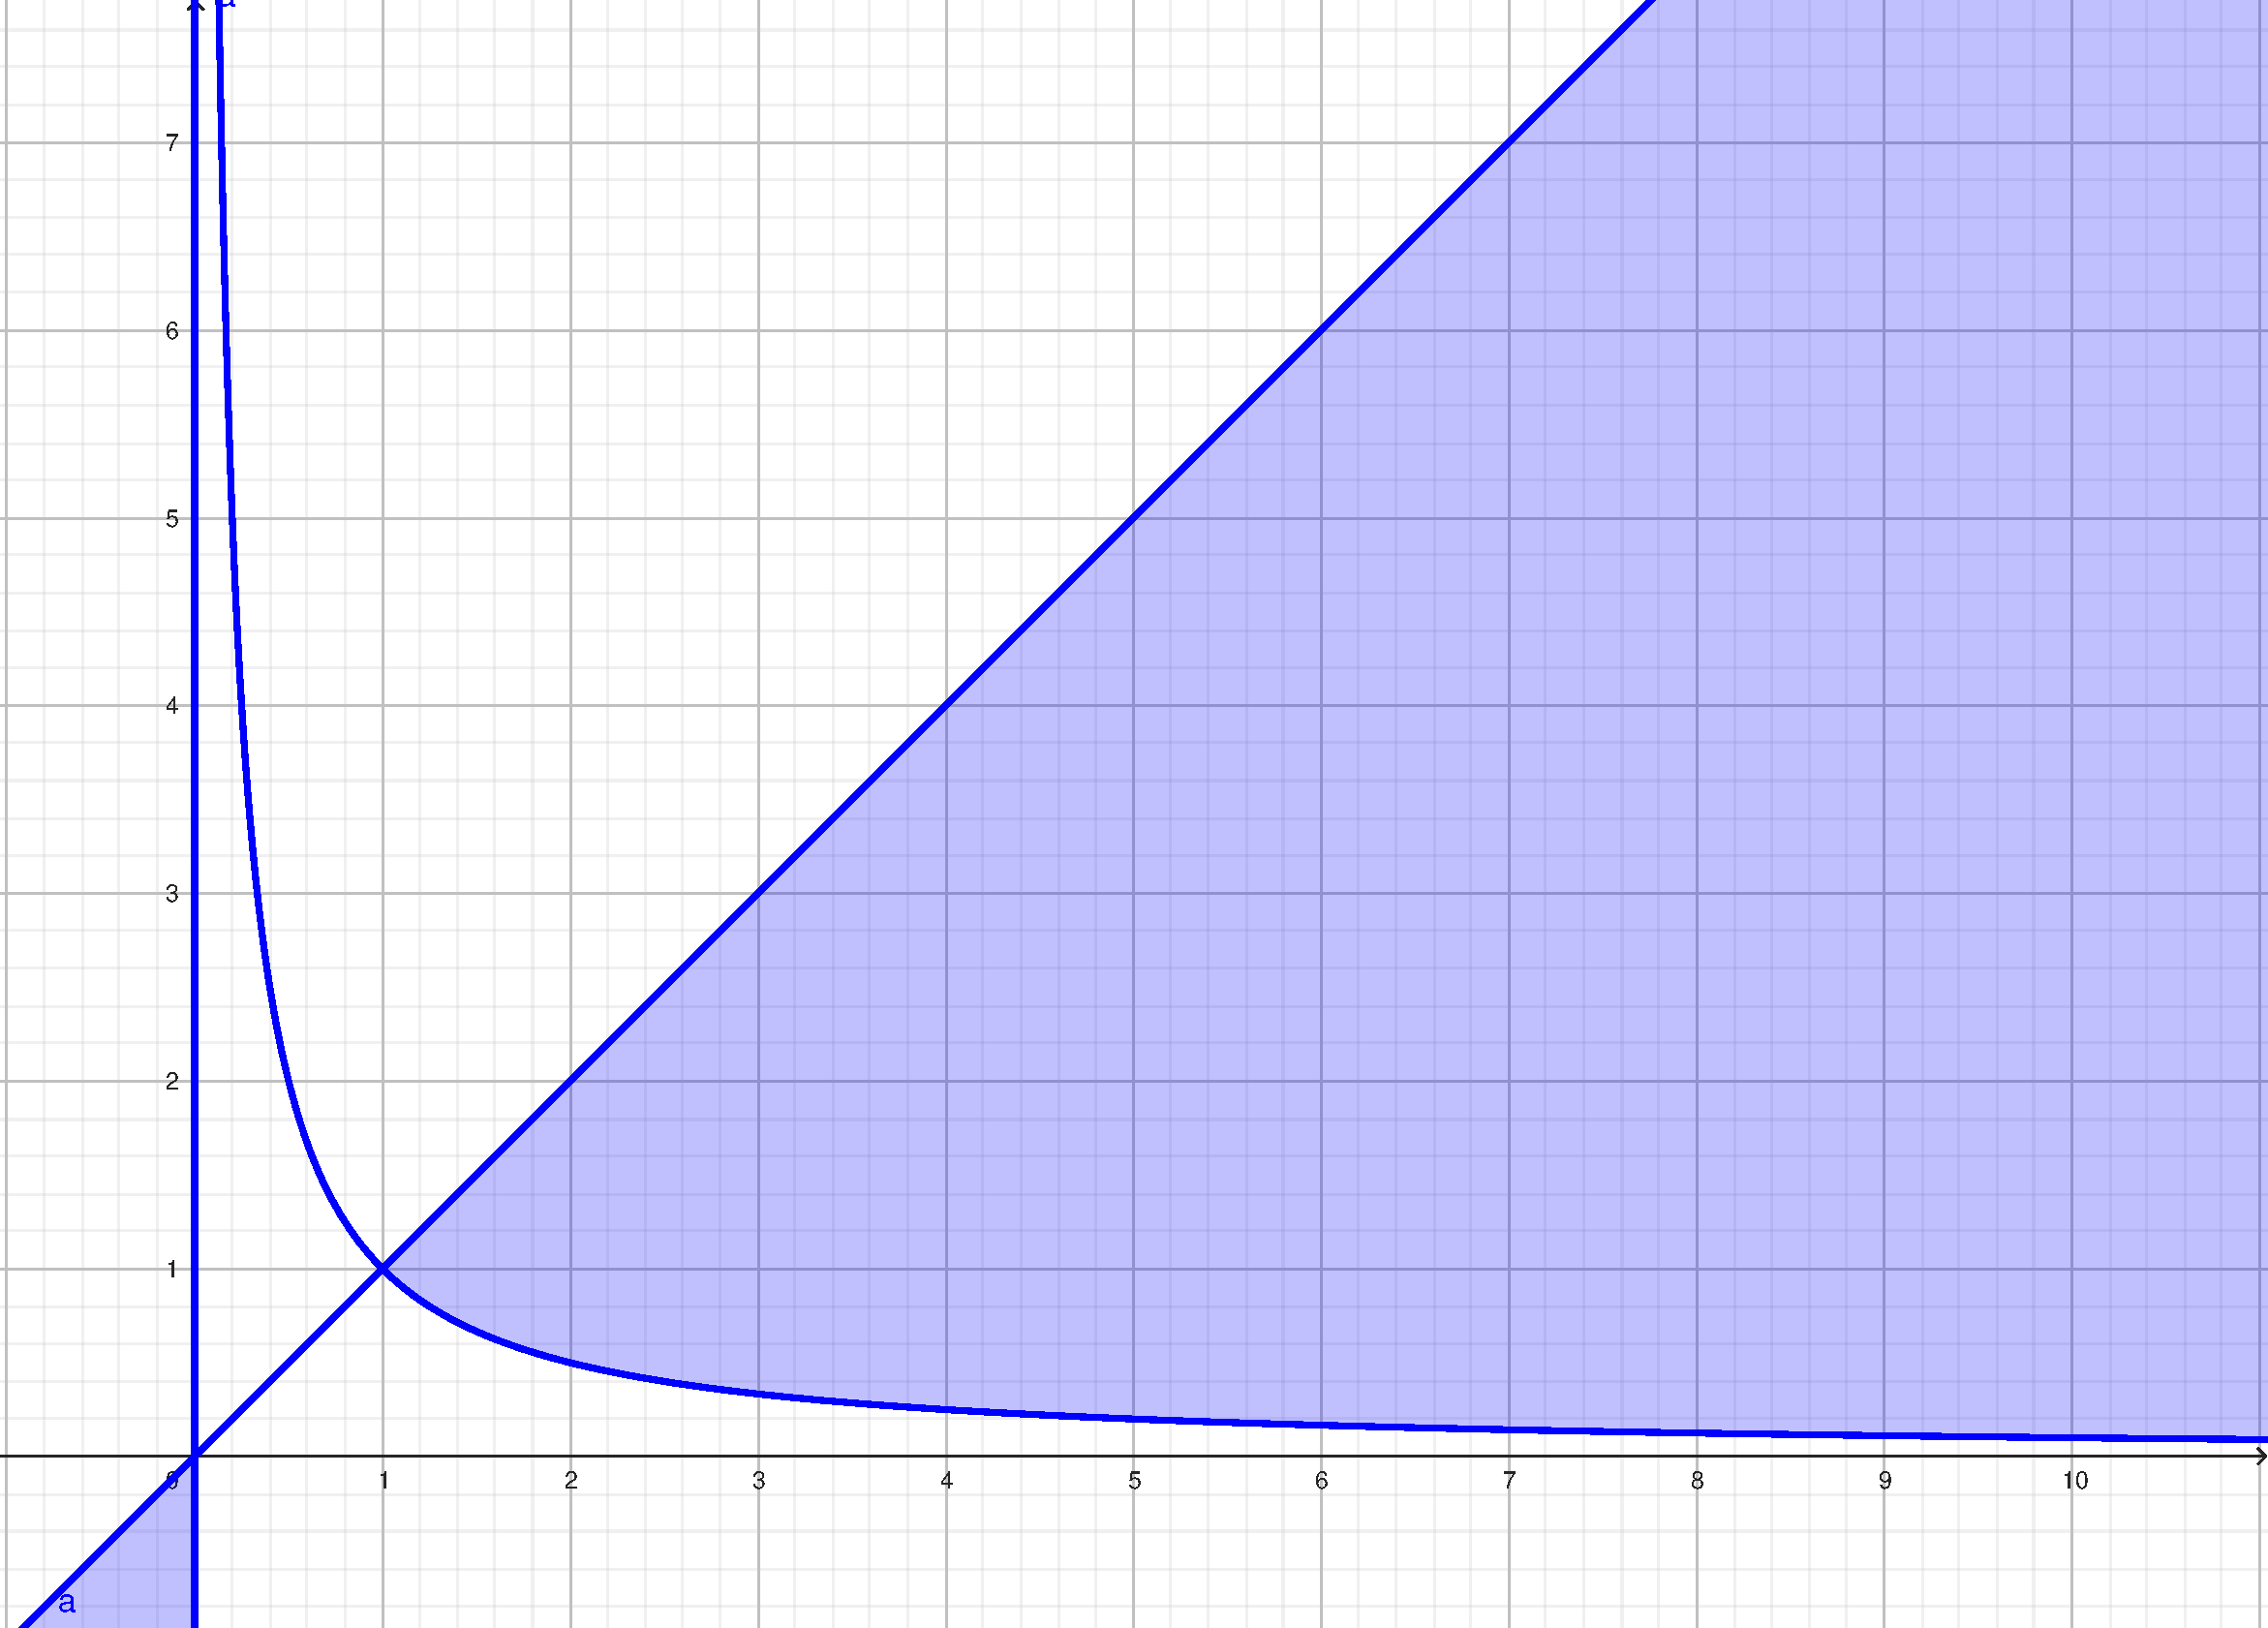
\includegraphics[scale=.15]{p78-14}
    \end{figure}

    设积分区域(阴影部分)为$D$,则将$D$投影到$y$轴上.\href{https://en.wikipedia.org/wiki/Multiple_integral#Normal_domains_on_R2}{(复习)}
    \leftnote{\color{red}此处的$x$的范围并不是$[1,+\infty]$.应将$D$投影到$y$轴上来讨论$x$的范围(\textit{想累次积分定义})}
    \[D = D_1 + D_2 = \{x\geq y, 1\leq y\} + \{x\geq 1/y , 0< y \leq 1\}\]
    \begin{align*}
        \ie\quad f_Y(y) & = \int_{D_1}f(x,y)\dd{x} + \int_{D_2}f(x,y)\dd{x}                                       \\
                        & =\begin{cases}
                               \displaystyle\int_{1/y}^{+\infty}\dfrac{1}{2x^2y}\dd{x}, 0< y\leq 1, \\
                               \displaystyle\int_{y}^{+\infty}\dfrac{1}{2x^2y}\dd{x}, 1\leq y,      \\
                               \displaystyle 0, \hphantom{;;\int_{y}^{+\infty}\dfrac{1}{2x^2y}}\text{else}
                           \end{cases}
                        & = (\cdots)
    \end{align*}
    \leftnote{要写出乘积.若判断独立性先枚举特值找反例.}
    两者相乘,显然不与$f(x,y)$相等.\;\;$\tf\; XY$不独立.
}
\end{document}